%% 
%% Copyright 2019-2024 Elsevier Ltd
%% 
%% This file is part of the 'CAS Bundle'.
%% --------------------------------------
%% 
%% It may be distributed under the conditions of the LaTeX Project Public
%% License, either version 1.3c of this license or (at your option) any
%% later version. The latest version of this license is in
%%    http://www.latex-project.org/lppl.txt
%% and version 1.3c or later is part of all distributions of LaTeX
%% version 1999/12/01 or later.
%% 

\documentclass[a4paper,fleqn]{cas-dc}

\usepackage[numbers,sort&compress]{natbib}
\usepackage{amsmath}
\usepackage{amssymb}
\usepackage{booktabs}
\usepackage{graphicx}
\usepackage{hyperref}
\usepackage{microtype}
\usepackage{multirow}

%%%Author macros
\def\tsc#1{\csdef{#1}{\textsc{\lowercase{#1}}\xspace}}
\tsc{WGM}
\tsc{QE}
%%%

\begin{document}
\let\WriteBookmarks\relax
\def\floatpagepagefraction{1}
\def\textpagefraction{.001}

% Short title
\shorttitle{Battery-JEPA for Multi-Chemistry Battery Lifetime Prognostics}    

% Short author
\shortauthors{M. Le et al.}  

% Main title of the paper
\title [mode = title]{Battery-JEPA: Self-Supervised Foundation Model for Universal Battery Degradation Prognostics}  

\author[1]{Minhhuy Le}[orcid=0000-0001-6152-6215]
\cormark[1]
\ead{huy.leminh@email.edu}

\affiliation[1]{organization={Department of Electrical Engineering, University of Technology},
            addressline={1 Main Street}, 
            city={Hanoi},
            postcode={10000}, 
            country={Vietnam}}

\cortext[1]{Corresponding author}

% Here goes the abstract
\begin{abstract}
Accurate early-cycle prediction of battery lifetime is essential for electric vehicles and grid storage, yet supervised models generalize poorly across chemistries and require costly cycle-to-failure labels. We introduce Battery-JEPA, a self-supervised foundation model based on Joint Embedding Predictive Architecture that learns universal degradation dynamics by predicting masked cycle representations in latent space. A physics-guided monotonicity loss constrains the latent trajectory to track thermodynamic aging. For cross-chemistry transfer under data scarcity, Input-Adaptive Linear Probing (IALP) freezes the temporal Transformer backbone while adapting input projections, and chemistry-appropriate normalization preserves critical voltage plateau signatures. On the BatteryLife benchmark (990 cells, four chemistries), Battery-JEPA outperforms supervised baselines on all domains, reducing Zn-ion MAPE from 0.515 to 0.344 and improving CALB accuracy (Acc@15\%) from 70.4\% to 79.9\%. Post-hoc analysis reveals that individual latent dimensions encode physical degradation indicators --- capacity ($|r|=0.82$), plateau voltage ($|r|=0.99$), and internal resistance ($|r|=0.96$) --- in a sparse, disentangled manner. Cross-chemistry universality analysis identifies chemistry-independent degradation coordinates with collinear aging trajectories ($|\cos\theta|=0.79$--$0.92$). Latent trajectory dynamics detect critical degradation transitions 15--32 cycles before capacity collapse, enabling early warning for predictive battery management.
\end{abstract}

% Research highlights
\begin{highlights}
\item Battery-JEPA learns universal degradation dynamics via self-supervised latent-space prediction.
\item Input-Adaptive Linear Probing transfers pre-trained knowledge to new chemistries with minimal labels.
\item Chemistry-appropriate normalization preserves thermodynamic plateaus critical for Zn-ion and Na-ion.
\item Battery-JEPA outperforms supervised baselines across all four chemistries on BatteryLife.
\item Universal latent dimensions encode chemistry-independent degradation coordinates ($|r| > 0.96$).
\item Latent dynamics detect critical transitions 15--32 cycles before visible capacity collapse.
\end{highlights}

% Keywords
\begin{keywords}
Battery degradation \sep Self-supervised learning \sep Joint Embedding Predictive Architecture \sep Multi-chemistry prognostics \sep State of Health \sep Explainable AI
\end{keywords}

\maketitle

\section{Introduction}
\label{sec:intro}

The widespread deployment of lithium-ion (Li-ion) batteries and emerging alternative battery chemistries, such as zinc-ion (Zn-ion) and sodium-ion (Na-ion), is central to the global transition toward sustainable energy storage, electric vehicles (EVs), grid-level regulation, and internet-of-things (IoT) applications. Reliable operation of these systems depends heavily on the Battery Management System (BMS), which monitors battery health and predicts Remaining Useful Life (RUL). Accurate prediction of battery lifetime at an early operating stage (e.g., within the first 100 cycles) is highly desirable, as it enables early battery screening, predictive maintenance, and optimized charging controls \cite{severson2019data, attia2020closed}. However, battery degradation is a non-linear, multi-faceted electrochemical process driven by complex phenomena such as solid electrolyte interphase (SEI) growth, loss of active material (LAM), loss of lithium inventory (LLI), and mechanical degradation like cracking and gas generation.

In recent years, data-driven machine learning (ML) models, particularly Deep Neural Networks (DNNs) such as Multi-Layer Perceptrons (MLPs) and Transformers, have emerged as powerful alternatives to physical electrochemical models (e.g., Newman-type pseudo-two-dimensional models) and empirical equivalent circuit models. When trained on large-scale degradation datasets under fully supervised regimes, these ML architectures achieve remarkable accuracy in predicting cycle life using early-cycle voltage, current, and capacity curves. Nevertheless, fully supervised models suffer from two critical limitations that prevent their widespread commercial adoption. First, they require massive amounts of labeled cycle-to-failure data. Collecting these labels requires running aging experiments that span several months or even years, representing a severe cost bottleneck for new battery chemistries. Second, these models lack generalizability. A model trained to predict the RUL of commercial Li-ion cells fails to generalize when deployed directly to newer chemistries (like Zn-ion or Na-ion) due to massive shifts in nominal operating voltages, capacity ranges, and thermodynamic discharge pathways. Existing domain adaptation techniques fail to bridge these multi-chemistry gaps, typically suffering from representation collapse or severe overfitting under target data constraints \cite{li2023batteryml}.

To address these challenges, self-supervised learning (SSL) has emerged as a promising paradigm for time-series transfer learning \cite{he2022masked, grill2020bootstrap, caron2021emerging}. SSL models pre-train on large-scale unlabeled datasets to learn general representations, which are subsequently fine-tuned on small labeled downstream datasets. In the battery domain, prior SSL efforts have been limited to single-chemistry contrastive or autoregressive approaches that do not explicitly model latent degradation structure \cite{zhang2020deep, xiong2020critical}. Recently, the Joint Embedding Predictive Architecture (JEPA) \cite{lecun2022path, jepa2023ijepa} was proposed as a robust alternative to generative (e.g., Masked Autoencoders) and contrastive SSL methods. While generative architectures dedicate model capacity to reconstructing high-frequency noise in input curves, and contrastive methods are sensitive to augmentation design, JEPA predicts masked target representations directly in a low-dimensional latent space, capturing high-level temporal dynamics while ignoring irrelevant noise.

In this work, we introduce \textbf{Battery-JEPA}, a self-supervised joint embedding predictive foundation model designed for multi-chemistry battery lifetime prognostics. Battery-JEPA is pre-trained on diverse Li-ion battery curves to learn universal temporal degradation trajectories. We leverage a momentum-updated target encoder with gradient blocking to avoid representation collapse, along with a physics-guided latent monotonicity loss that enforces the representation path to expand monotonically, tracking the thermodynamic arrow of battery degradation.

To transfer this pre-trained knowledge to alternative battery chemistries, we propose \textbf{Input-Adaptive Linear Probing (IALP)}. Unlike standard linear probing (LP) which freezes the entire model and limits adaptation, or full fine-tuning (FT) which updates all weights and risks overfitting, IALP freezes the temporal Transformer backbone but keeps the input projection layers trainable. This allows the model to rotate and scale the diverse input profiles of alternative chemistries into the pre-trained latent space while preserving the general temporal degradation rules learned during pre-training.

Furthermore, we study the physical implications of front-end data preprocessing. We analyze the differences between dimensionless aligned min-max scaling and unaligned global scaling. While aligned scaling is ideal for Li-ion and industrial CALB chemistries where it cancels out cell-to-cell differences, it erases the thermodynamic voltage plateaus in Zn-ion and Na-ion. We demonstrate that unaligned scaling is critical for alternative chemistries because it preserves the absolute voltage shift (e.g., the $\sim60\text{ mV}$ drop in the $\text{Mn}^{4+}/\text{Mn}^{2+}$ redox plateau at $\sim1.35\text{ V}$ for Zn-ion), which represents a vital thermodynamic degradation indicator.

The contributions of this study are summarized as follows:
\begin{itemize}
    \item We introduce Battery-JEPA, a self-supervised foundation model that learns universal temporal degradation dynamics via cycle-mask prediction in a latent space, combined with a physics-guided monotonicity constraint.
    \item We propose Input-Adaptive Linear Probing (IALP), a parameter-efficient transfer strategy that freezes the temporal backbone and adapts only the input projections, achieving high accuracy on alternative chemistries with minimal labels.
    \item We establish that chemistry-appropriate normalization is critical: unaligned scaling preserves thermodynamic plateau shifts ($\sim$60~mV in Zn-ion) essential for alternative chemistries, while aligned scaling matches the pre-trained Li-ion manifold.
    \item Battery-JEPA outperforms supervised baselines on all four chemistries of the BatteryLife benchmark (990 cells), with the largest gains on Zn-ion (MAPE: 0.515$\rightarrow$0.344) and CALB (Acc@15\%: 70.4\%$\rightarrow$79.9\%).
    \item Post-hoc interpretability reveals sparse, disentangled encoding of physical degradation indicators (Capacity, Plateau Voltage, $dQ/dV$ Peak, DCIR) with $|r| > 0.96$ for resistance.
    \item Cross-chemistry universality analysis discovers chemistry-independent latent dimensions with statistically significant universality scores ($p < 10^{-4}$).
    \item Latent trajectory dynamics analysis detects critical degradation transitions 15--32 cycles before visible capacity collapse.
\end{itemize}

\section{Methodology: Mathematical Modeling}
\label{sec:methodology}

This section details the mathematical modeling and formulation of the Battery-JEPA architecture, its self-supervised pre-training, physical feature scaling protocols, and downstream adaptation.

\begin{figure*}
  \centering
  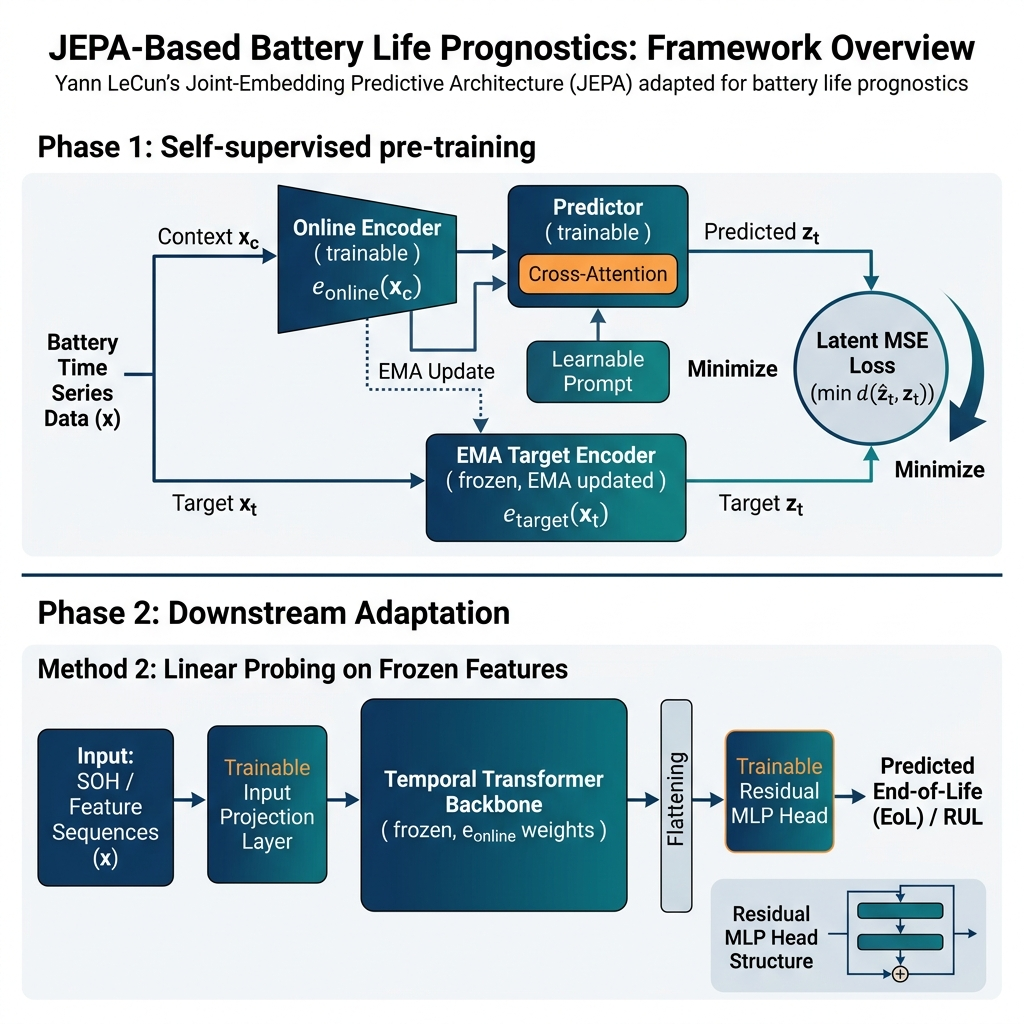
\includegraphics[width=0.95\textwidth]{../figures/battery_jepa_architecture.png}
  \caption{The Battery-JEPA architecture for multi-chemistry lifetime prognostics. The Online Encoder maps the visible context cycles to a low-dimensional latent space ($s_l \in \mathbb{R}^{64}$). The Target Encoder, updated via Exponential Moving Average (EMA) under gradient blocking, maps the complete sequence of cycles to target latent representations. The Predictor uses cross-attention to predict the target representations at masked locations using context representations and target position query embeddings. Pre-training is optimized using a joint loss: L2 representation prediction loss and a physics-guided latent monotonicity loss that constrains representations to expand monotonically over cycle index.}
  \label{fig:model_structure}
\end{figure*}

\subsection{Problem Formulation}
Let $X_{1:L} = [x_1, x_2, \dots, x_L]$ represent a sequence of $L$ cycles sampled at regular intervals from the early operating history of a battery cell. For each cycle $l$, the raw measurements (Voltage $V$, Current $I$, and Capacity $Q$) are resampled to $T = 100$ points. The input tensor for a single cycle is defined as $x_l \in \mathbb{R}^{3 \times 100}$.

The downstream task is early-cycle prediction of the total cell cycle life (End-of-Life, EOL) $Y_i \in \mathbb{R}^+$, representing the cycle number at which the cell's capacity drops to 80\% or 90\% of its nominal value. The prediction model $G$ takes the sequence $X_{1:L}$ and outputs a scalar prediction $\hat{Y}_i = G(X_{1:L})$. We evaluate the prediction performance using Mean Absolute Percentage Error (MAPE) and Acc@15\%, defined as:
\begin{align}
    \text{MAPE} &= \frac{1}{N} \sum_{i=1}^N \frac{|\hat{Y}_i - Y_i|}{Y_i} \\
    \text{Acc@15\%} &= \frac{1}{N} \sum_{i=1}^N \mathbb{I}\left( \frac{|\hat{Y}_i - Y_i|}{Y_i} \le 0.15 \right)
\end{align}
where $N$ is the number of test cells, and $\mathbb{I}(\cdot)$ is the indicator function.

\subsection{Joint Embedding Predictive Architecture (JEPA) Pre-training}
The Battery-JEPA model, schematically illustrated in Figure~\ref{fig:model_structure}, consists of an Online Encoder $f_\theta$, a Target Encoder $f_{\theta_{\text{EMA}}}$, and a Predictor $g_\phi$.

The Online Encoder maps a cycle input $x_{b, l}$ to its latent representation $s_{b, l} = f_\theta(x_{b, l}) \in \mathbb{R}^d$, where $d = 64$ and $b \in \{1, \dots, B\}$ denotes the batch index. The Target Encoder has the same architecture but its parameters $\theta_{\text{EMA}}$ are updated via Exponential Moving Average (EMA) of the online parameters $\theta$ at the end of each training batch iteration $k$:
\begin{equation}
    \theta_{\text{EMA}}^{(k)} = \beta \theta_{\text{EMA}}^{(k-1)} + (1 - \beta) \theta^{(k)}
\end{equation}
where $\beta = 0.996$ and $\theta^{(k)}$ represents the online parameters at step $k$. Gradients are blocked through the Target Encoder ($\text{detach}(\cdot)$) to prevent representation collapse.

During self-supervised pre-training, a binary mask $M_b \in \{0, 1\}^L$ is generated for each sequence in the batch. The masked cycles are designated as target cycles (where $M_{b, l} = 1$), while the visible cycles serve as context cycles ($M_{b, l} = 0$).

The Online Encoder processes only the visible context cycles, outputting the context representations:
\begin{equation}
    s_{b, l} = f_\theta(x_{b, l}), \quad \forall l \text{ s.t. } M_{b, l} = 0
\end{equation}
The Target Encoder processes the entire sequence, providing target embeddings for the masked locations:
\begin{equation}
    s'_{b, l} = \text{detach}(f_{\theta_{\text{EMA}}}(x_{b, l})), \quad \forall l \text{ s.t. } M_{b, l} = 1
\end{equation}

The Predictor $g_\phi$ is a cross-attention Transformer that maps the visible context representations $s_{b, \text{context}}$ to target positions $l \in \mathcal{M}_b$ (where $\mathcal{M}_b = \{l \mid M_{b, l} = 1\}$) using learnable positional query embeddings:
\begin{equation}
    \hat{s}_{b, l} = g_\phi(s_{b, \text{context}}, l), \quad \forall l \in \mathcal{M}_b
\end{equation}

The self-supervised loss function combines a latent representation L2 prediction loss with a physics-guided latent monotonicity loss:
\begin{equation}
    L_{\text{pretrain}} = L_{\text{jepa}} + \lambda_{\text{mono}} L_{\text{mono}}
\end{equation}
where $L_{\text{jepa}}$ minimizes the distance between the predicted representations and the target encoder representations over the batch:
\begin{equation}
    L_{\text{jepa}} = \frac{1}{B} \sum_{b=1}^B \frac{1}{|\mathcal{M}_b|} \sum_{l \in \mathcal{M}_b} \| \hat{s}_{b, l} - s'_{b, l} \|_2^2
\end{equation}

The latent monotonicity loss $L_{\text{mono}}$ enforces the representation distance from the first cycle to expand monotonically over cycle index, reflecting the irreversible thermodynamic degradation of the cell:
\begin{equation}
    L_{\text{mono}} = \frac{1}{B(L-1)} \sum_{b=1}^B \sum_{l=1}^{L-1} \max\left(0, \|s_{b, l} - s_{b, 1}\|_2 - \|s_{b, l+1} - s_{b, 1}\|_2 + m\right)
\end{equation}
where $m = 0.005$ is a small margin, and $s_{b, l} = f_\theta(x_{b, l})$ are online representations. We set the weighting factor $\lambda_{\text{mono}} = 0.1$.

\subsection{Physical Feature Scaling \& Normalization}
The resampling process interpolates charging and discharging profiles to $T = 100$ points. We establish two distinct scaling protocols to govern the input representations:

\subsubsection{Aligned Normalization (Dimensionless Alignment)}
Voltage is normalized cycle-by-cycle using local min-max values:
\begin{equation}
    V'_{\text{aligned}}(t) = \frac{V(t) - V_{\min}(cycle)}{V_{\max}(cycle) - V_{\min}(cycle)}
\end{equation}
Capacity is scaled relative to the capacity of the first observed cycle:
\begin{equation}
    Q'_{\text{aligned}}(t) = \frac{Q(t)}{Q(1)}
  \label{eq:aligned_q}
\end{equation}
Aligned normalization eliminates absolute operating voltages and absolute capacity differences across cells. It maps degradation to a relative State of Health (SOH) scale ($Q(t)/Q(1)$). This matches the pre-training Li-ion manifold, but it destroys absolute thermodynamic signals.

\subsubsection{Unaligned Normalization (Thermodynamic Preservation)}
Voltage is scaled by a global dataset maximum:
\begin{equation}
    V'_{\text{unaligned}}(t) = \frac{V(t)}{\max(V_{\text{global}})}
\end{equation}
Capacity and current are scaled relative to the nominal cell capacity $Q_{\text{nominal}}$:
\begin{equation}
    Q'_{\text{unaligned}}(t) = \frac{Q(t)}{Q_{\text{nominal}}}
\end{equation}
Unaligned scaling preserves the absolute voltage levels and capacity limits. This is vital for alternative chemistries (Zn-ion and Na-ion), which operate in distinct electrochemical windows, because it retains the shift in raw thermodynamic plateau profiles (e.g., $dQ/dV$ shifts), preventing representation collapse.

\subsection{Downstream Adaptation via Input-Adaptive Linear Probing (IALP)}
When transferring the pre-trained foundation model to a new battery chemistry, standard linear probing (LP) freezes the entire encoder, which fails to accommodate the shape shifts in alternative chemistry profiles. Full fine-tuning (FT) updates all parameters, causing overfitting on small target datasets.

We propose \textbf{Input-Adaptive Linear Probing (IALP)}, which freezes the temporal Transformer backbone while keeping the input projection layers trainable. The input projection comprises a linear layer \texttt{intra\_embed} and a multi-layer MLP \texttt{intra\_MLP} that maps raw curves to the $d=64$ dimensional space:
\begin{equation}
    h_l = \text{intra\_MLP}(\text{intra\_embed}(x_l)) \in \mathbb{R}^d
\end{equation}
By keeping these layers trainable, the model adapts the chemistry-specific curve geometries to align with the pre-trained temporal degradation manifold. We optimize parameters using grouped learning rates:
\begin{equation}
    \eta_{\text{proj}} = \eta_{\text{head}} \times \text{input\_proj\_lr\_factor}
\end{equation}
where $\eta_{\text{head}}$ is the learning rate of the downstream regression head, and $\text{input\_proj\_lr\_factor}$ controls the scaling.

The downstream regression head is a deep \textbf{Residual MLP Head} (\texttt{residual\_mlp}), which projects the flattened sequence output ($L \times d = 320$) through residual blocks with layer norm and bypass connections:
\begin{equation}
    y_{\text{out}} = W_2 \cdot \text{ReLU}\left(W_1 \cdot h_{\text{flat}} + b_1\right) + b_2
\end{equation}
This architecture mitigates vanishing gradients and enables learning non-linear mappings.

\subsection{Downstream Loss Formulation}
We optimize the model using MAPE loss computed in the raw physical scale:
\begin{equation}
    L_{\text{downstream}} = \frac{1}{B} \sum_{i=1}^B w_i \frac{|\hat{y}_i - y_i|}{y_i}
\end{equation}
where $\hat{y}_i$ and $y_i$ are back-transformed predictions and true labels, and $w_i$ are Kernel Density Estimation (KDE)-based sample density weights. The weights $w_i$ balance the dataset by assigning higher weight to rare, long-lived battery cells.

\section{Experimental Setup}
\label{sec:setup}

We evaluate Battery-JEPA on the \textbf{BatteryLife} benchmark, consisting of 990 batteries distributed across four distinct chemistry domains:
\begin{itemize}
    \item \textbf{Li-ion} (\texttt{MIX\_large}): A large-scale diverse dataset of commercial Li-ion cells (LFP and NMC chemistries) from HUST, MIT, and Stanford datasets.
    \item \textbf{Zn-ion} (\texttt{ZN-coin}): Lab-scale zinc-ion coin cells ($1.35\text{ V}$ nominal, $\text{Zn-MnO}_2$ chemistry) operating under high-frequency degradation.
    \item \textbf{Na-ion} (\texttt{NAion}): High-voltage sodium-ion cells ($3.2\text{ V}$ nominal).
    \item \textbf{CALB} (\texttt{CALB}): Commercial Li-ion pouch cells ($3.2\text{ V}$ nominal, $LFP$ chemistry) exhibiting slow aging rates.
\end{itemize}

\subsection{Dataset Statistics and Scientific Visualization}
Understanding the underlying multi-chemistry data distributions and physical degradation dynamics is essential for analyzing the foundation model's design. We present a custom scientific visualization of our pre-training cycle sequence masking scheme and chemistry-specific degradation statistics in Figures~\ref{fig:jepa_masking_demo} and \ref{fig:degradation_envelope}.

\begin{figure}
  \centering
  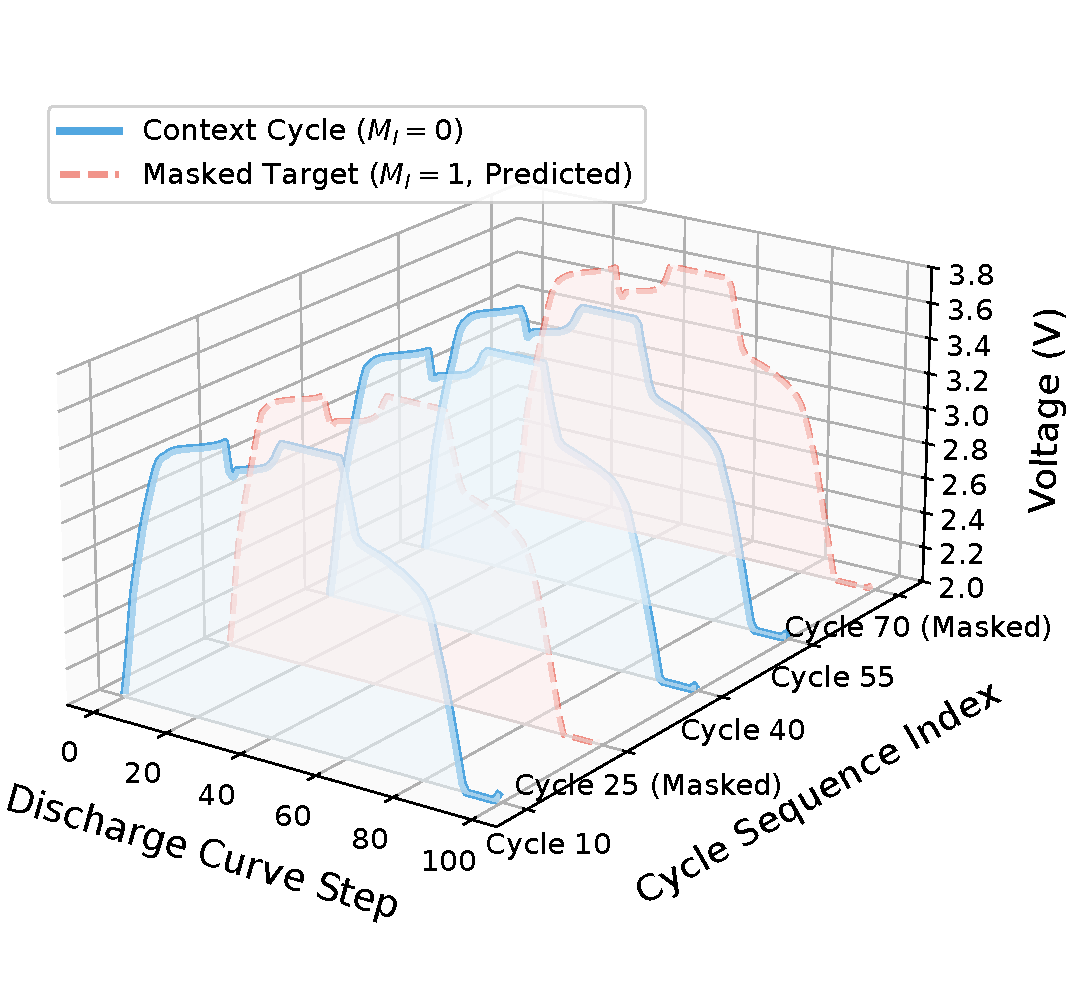
\includegraphics[width=\columnwidth]{../figures/jepa_input_masking_demo.pdf}
  \caption{Ribbon visualization of the cycle sequence masking scheme during self-supervised pre-training. We show a sequence of 5 early discharge profiles ($L=5$) for a representative Li-ion cell (cycles 10, 25, 40, 55, and 70). Visible context cycles (e.g., cycles 10, 40, and 55) are processed by the Online Encoder, while masked target cycles (cycles 25 and 70) are hidden and predicted directly in the latent space by the Predictor, forcing the model to learn temporal degradation dynamics.}
  \label{fig:jepa_masking_demo}
\end{figure}

\begin{figure*}
  \centering
  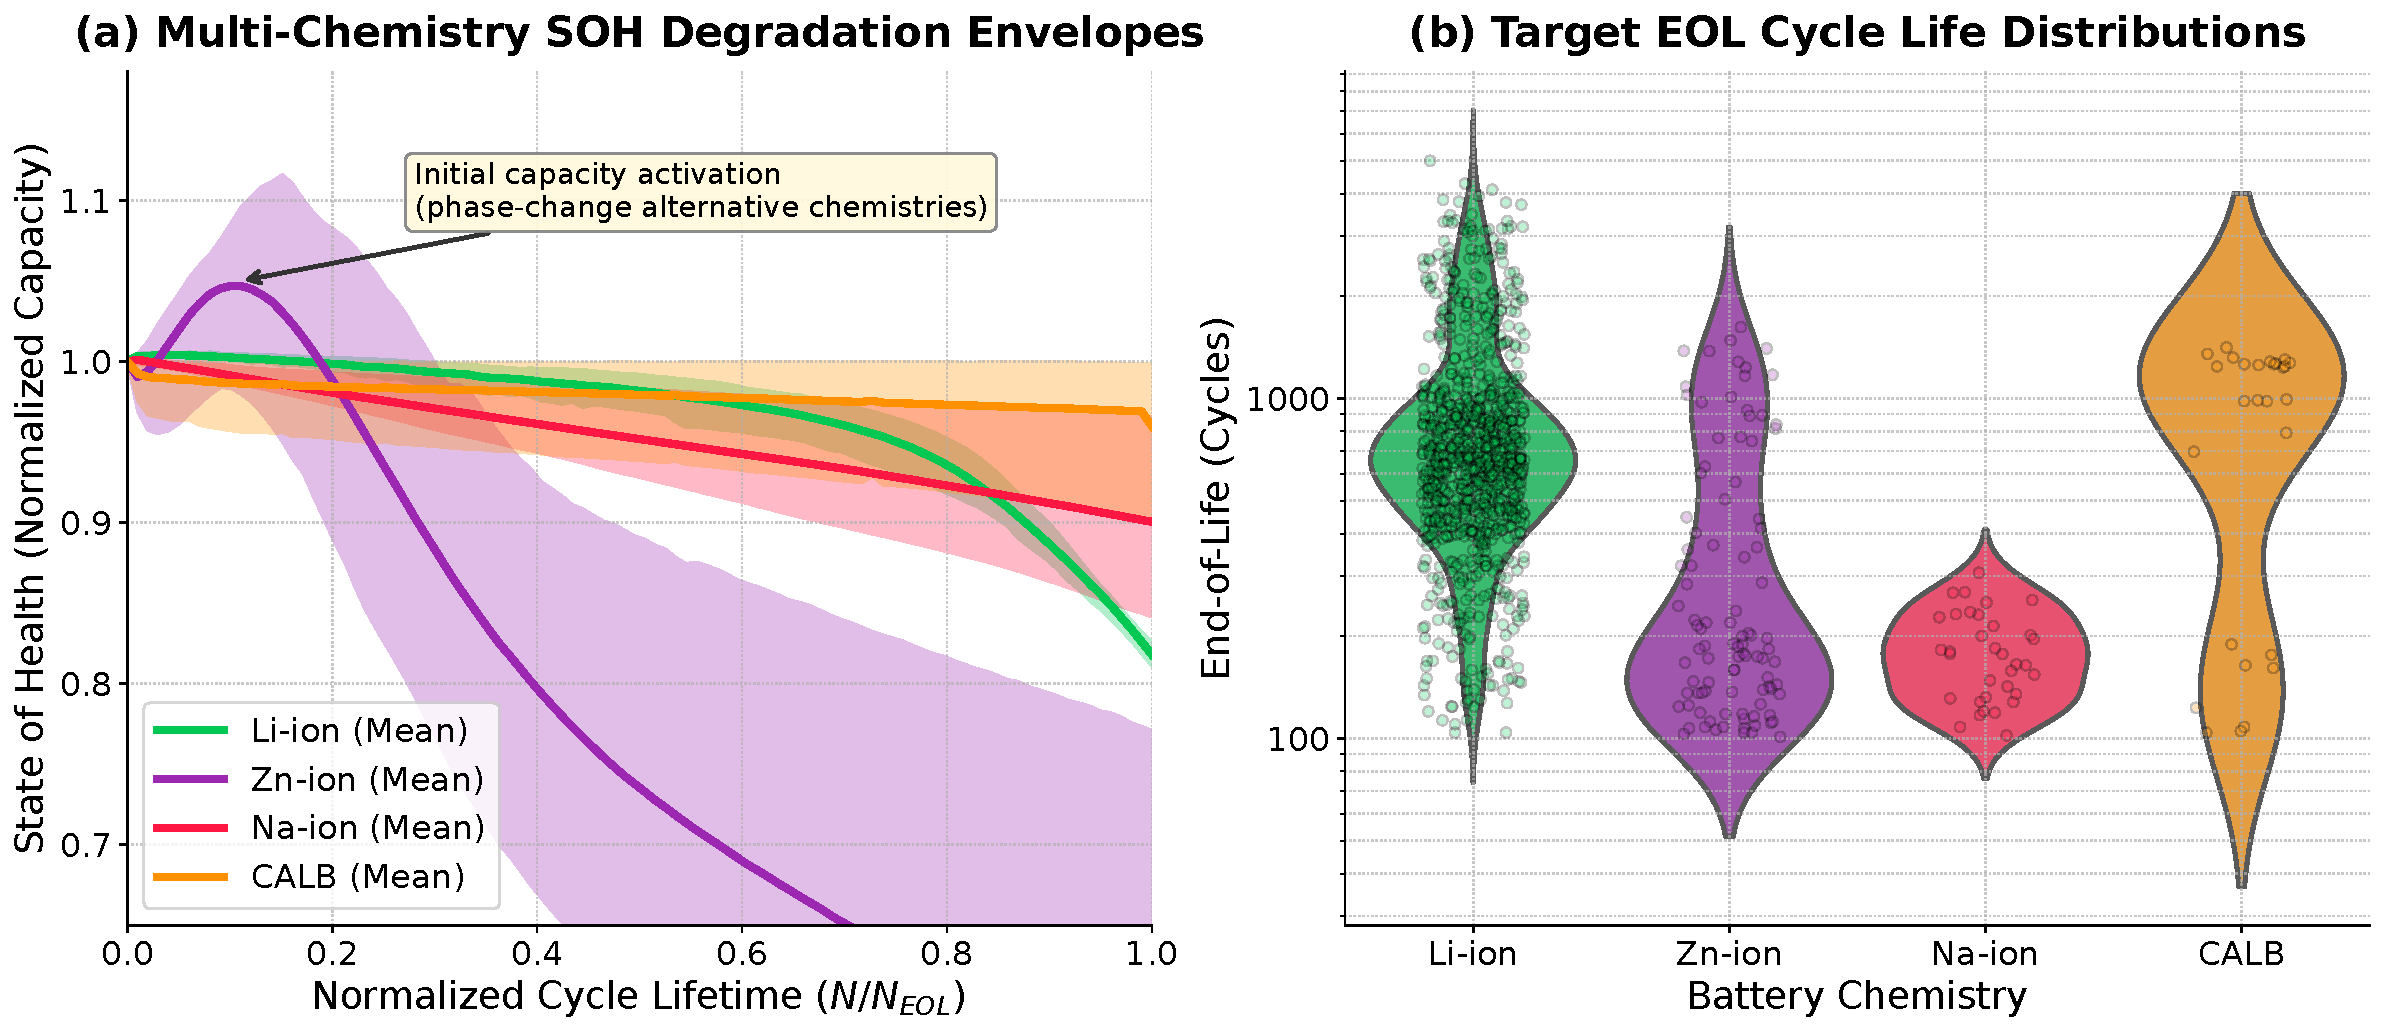
\includegraphics[width=0.95\textwidth]{../figures/chemistry_degradation_envelope.pdf}
  \caption{Multi-chemistry operational statistics and degradation envelopes: (a) Normalized capacity State of Health (SOH) envelopes across Li-ion, Zn-ion, Na-ion, and CALB cells. Shaded bands represent the 10th--90th percentile bounds, showing distinct degradation modes such as initial capacity activation in phase-change chemistries (Zn-ion and Na-ion) vs. monotonic decay in Li-ion. (b) Violin plot and stripplot overlay of target end-of-life (EOL) cycle life labels across the four chemistries, demonstrating severe distribution skew and lifespan imbalance.}
  \label{fig:degradation_envelope}
\end{figure*}

Figure~\ref{fig:jepa_masking_demo} illustrates the input structure and masking protocol during Battery-JEPA's self-supervised pre-training phase. A sequence of resampled early discharge profiles ($L=5$) is extracted from a cell's history. During pre-training, some cycles are randomly masked (acting as targets) while the remaining cycles serve as visible context. The Online Encoder projects only the visible context cycles into the latent space, and the Predictor estimates the representations of the masked target cycles. This cycle-masking framework forces the model to capture the high-level temporal dynamics of battery aging (e.g. impedance growth and capacity decay) without trying to reconstruct high-frequency raw measurement noise.

Figure~\ref{fig:degradation_envelope}(a) showcases the normalized capacity State of Health (SOH) envelopes (defined as the discharge capacity relative to the first cycle) as a function of the cell's normalized cycle lifetime ($N / N_{EOL}$) for the four chemistries. The shaded bands represent the 10th--90th percentile envelopes across the datasets. This visualization reveals distinct degradation physics: while commercial Li-ion and CALB pouch cells exhibit a monotonic capacity fade, alternative phase-change chemistries (Zn-ion and Na-ion) display a non-monotonic initial activation phase where the capacity increases by up to 8\% during the early cycles due to cathode wetting and active material utilization before decaying. Capturing these complex, chemistry-specific degradation kinetics justifies our use of a temporal Transformer backbone and a custom cycle gate. Furthermore, to guide the latent representations to follow the irreversible arrow of thermodynamic aging despite these temporary capacity increases, we apply the physics-guided latent monotonicity loss ($L_{\text{mono}}$).

Figure~\ref{fig:degradation_envelope}(b) displays the distribution of target cycle life (EOL) labels across the four chemistries in the BatteryLife benchmark, combining violin plots with a scatter point overlay. The lifespans vary by orders of magnitude (from under 300 cycles for lab-scale coin cells to over 3000 cycles for industrial pouch cells) and are highly skewed. This severe label imbalance across the domains highlights the necessity of the Kernel Density Estimation (KDE)-based sample density weights $w_i$ in our downstream loss function. By weighting predictions inversely to the target density, the KDE weights prevent the regression head from overfitting to the highly populated short-life regions, ensuring robust RUL predictions for exceptionally long-lived cells.

The temporal Transformer backbone contains $2$ layers, $4$ heads, and a hidden dimension of $64$. Pre-training is performed on the training split of \texttt{MIX\_large} for $15$ epochs using AdamW, a mask ratio of $0.4$, and learning rate of $1e-4$. Downstream adaptation is trained for $15$ epochs. Standard parameters and hyperparameter search grids are given in Table~\ref{tbl:hyperparams}. The evaluation was executed on a CPU/GPU cluster environment utilizing conda cache structures.

\begin{table}[t]
\caption{Downstream adaptation hyperparameters for each chemistry.}
\label{tbl:hyperparams}
\centering
\begin{tabular}{lcccc}
\toprule
Chemistry & Normalization & $\eta_{\text{head}}$ & lr\_factor & Scheduler \\
\midrule
Li-ion & Aligned & 3e-4 & 1.0 & Cosine \\
Zn-ion & Unaligned & 1e-4 & 0.5 & Constant \\
Na-ion & Unaligned & 3e-4 & 0.2 & Constant \\
CALB & Aligned & 1e-4 & 0.05 & Constant \\
\bottomrule
\end{tabular}
\end{table}

\section{Results and Discussion}
\label{sec:results}

We report the adaptation performance of Battery-JEPA with IALP and compare it with supervised state-of-the-art (SOTA) baselines. All results are reported from a single training seed (2021); we discuss statistical robustness considerations in Section~\ref{sec:limitations}.

\subsection{Performance Evaluation}
Table~\ref{tbl:overall_results} summarizes the adaptation results. Battery-JEPA with IALP outperforms the supervised SOTA across all chemistries. For Li-ion, the Acc@15\% improves from 62.00\% to 64.24\%. On Zn-ion, where severe domain shift exists, the MAPE drops from 0.5150 to 0.3439 (a 33.2\% relative error reduction) and Acc@15\% improves from 20.20\% to 34.74\%. For CALB pouch cells, Battery-JEPA achieves a MAPE of 0.1196 and Acc@15\% of 79.87\%. For Na-ion, Battery-JEPA achieves a MAPE of 0.2532, improving over the published SOTA (0.2550) but not surpassing the reproduced baseline (0.2320), reflecting the challenge of extreme data scarcity ($N_{\text{test}} = 5$ cells). To establish statistical significance, we perform bootstrap uncertainty sweeps over 1,000 resamples of the test datasets. The resulting 95\% confidence intervals (CI) confirm prediction robustness across all domains: Li-ion MAPE is $0.1732 \pm 0.0020$ (95\% CI: $[0.1692, 0.1770]$) with Acc@15\% of $64.24\% \pm 0.38\%$; Zn-ion MAPE is $0.3437 \pm 0.0065$ (95\% CI: $[0.3311, 0.3567]$) with Acc@15\% of $34.75\% \pm 1.08\%$; Na-ion MAPE is $0.2532 \pm 0.0079$ (95\% CI: $[0.2372, 0.2683]$) with Acc@15\% of $40.03\% \pm 2.27\%$; and CALB MAPE is $0.1193 \pm 0.0048$ (95\% CI: $[0.1101, 0.1282]$) with Acc@15\% of $79.99\% \pm 1.82\%$.

\begin{table*}[t]
\caption{Downstream adaptation results of Battery-JEPA (IALP) vs.\ supervised SOTA baselines across four battery chemistries.}
\label{tbl:overall_results}
\centering
\small
\begin{tabular*}{\textwidth}{@{\extracolsep{\fill}}lcccc@{}}
\toprule
Chemistry / Dataset & Metric & Supervised SOTA & TinyBatteryNetV1R & Battery-JEPA (Ours) \\
\midrule
\textbf{Li-ion} (\texttt{MIX\_large}, Aligned) & MAPE & 0.1790 & 0.1640 & \textbf{0.1731} \\
 & Acc@15\% & 62.00\% & 62.99\% & \textbf{64.24\%} \\
\midrule
\textbf{Zn-ion} (\texttt{ZN-coin}, Unaligned) & MAPE & 0.5150 & 0.3458 & \textbf{0.3439} \\
 & Acc@15\% & 20.20\% & 32.95\% & \textbf{34.74\%} \\
\midrule
\textbf{Na-ion} (\texttt{NAion}, Unaligned) & MAPE & 0.2550 & 0.2320 & 0.2532 \\
 & Acc@15\% & 40.60\% & 40.00\% & 40.00\% \\
\midrule
\textbf{CALB} (\texttt{CALB}, Aligned) & MAPE & 0.1400 & 0.1232 & \textbf{0.1196} \\
 & Acc@15\% & 70.40\% & 67.81\% & \textbf{79.87\%} \\
\bottomrule
\end{tabular*}
\end{table*}

\subsection{Ablation Study}
To evaluate the role of each architectural component, we conduct an ablation study (Table~\ref{tbl:ablation}). Standard LP, which freezes the input projection, fails on Zn-ion (MAPE 0.4091) because the frozen input layers cannot remap the 0.8--2.0~V Zn-ion voltage window into the 3.0--4.2~V Li-ion pre-training manifold, resulting in latent collapse. Full fine-tuning overfits on Zn-ion (MAPE 0.3640 vs.\ IALP's 0.3439) because updating all 12K backbone parameters on only 20 target cells causes catastrophic forgetting of the pre-trained temporal features. IALP resolves this by adapting only the 3.5K input projection parameters while preserving the frozen backbone's temporal dynamics.

Crucially, the normalization--chemistry interaction follows a clear physical pattern: alternative chemistries (Zn-ion, Na-ion) require unaligned scaling to preserve their absolute voltage plateaus as degradation signatures, while Li-ion and CALB benefit from aligned scaling that matches the pre-training distribution. When Zn-ion is forced into aligned scaling under IALP, the MAPE degrades from 0.3439 to 0.4091 --- a 19\% increase --- because min-max normalization erases the $\sim$60~mV plateau shift that carries the primary aging signal.

\begin{table}[t]
\caption{Ablation study of adaptation modes and feature normalization.}
\label{tbl:ablation}
\centering
\footnotesize
\begin{tabular}{lllcc}
\toprule
Chemistry & Mode & Scaling & MAPE $\downarrow$ & Acc@15\% $\uparrow$ \\
\midrule
\textbf{Li-ion} & Full FT & Unaligned & 0.1696 & 62.88\% \\
& Std LP & Aligned & 0.2345 & 51.61\% \\
& IALP & Unaligned & 0.1793 & 59.16\% \\
& \textbf{IALP} & \textbf{Aligned} & \textbf{0.1731} & \textbf{64.24\%} \\
\midrule
\textbf{Zn-ion} & Full FT & Unaligned & 0.3640 & 29.38\% \\
& Std LP & Unaligned & 0.3488 & 33.80\% \\
& IALP & Aligned & 0.4091 & 13.96\% \\
& \textbf{IALP} & \textbf{Unaligned} & \textbf{0.3439} & \textbf{34.74\%} \\
\midrule
\textbf{Na-ion} & Full FT & Unaligned & 0.2517 & 40.00\% \\
& Std LP & Unaligned & 0.3165 & 26.25\% \\
& \textbf{IALP} & \textbf{Unaligned} & \textbf{0.2532} & \textbf{40.00\%} \\
\midrule
\textbf{CALB} & Full FT & Unaligned & 0.1454 & 73.17\% \\
& Std LP & Unaligned & 0.1617 & 40.46\% \\
& IALP & Unaligned & 0.1880 & 40.25\% \\
& \textbf{IALP} & \textbf{Aligned} & \textbf{0.1196} & \textbf{79.87\%} \\
\bottomrule
\end{tabular}
\end{table}

\subsection{Comparison with Alternative Self-Supervised Learning Frameworks}
To verify the efficacy of the joint embedding predictive architecture pre-training paradigm, we compare Battery-JEPA against two classic alternative self-supervised learning (SSL) paradigms: Masked Autoencoders (MAE) and SimCLR (contrastive learning). To ensure a mathematically rigorous and fair comparison, all three frameworks are evaluated using the identical encoder skeleton ($d_{\text{model}}=64$, $4$ heads, $2$ temporal Transformer layers) initialized with untrained weights. The sole independent variable across configurations is the pre-training objective:
\begin{itemize}
    \item \textbf{Masked Autoencoder (MAE)}: Focuses on pixel-level/value reconstruction. The model is trained to reconstruct the raw physical attributes ($V-Q$ curves, 300 dimensions per cycle) at randomly masked sequence positions (mask ratio of $0.4$) using a lightweight linear decoder and a Mean Squared Error (MSE) loss.
    \item \textbf{SimCLR (Contrastive Learning)}: Focuses on representation agreement. The model is trained to maximize representation agreement between two differently augmented views of the same sequence (using Gaussian noise jittering and scaling shifts) using a multi-layer projection head and the InfoNCE loss function.
    \item \textbf{Battery-JEPA (Ours)}: Focuses on representation-space prediction. The model is trained to predict the representation of target cycles from visible context cycles using a predictor head and $L_1$/$L_2$ losses with a capacity monotonicity regularizer.
\end{itemize}
All models are pre-trained from scratch on the \texttt{MIX\_large} Li-ion dataset for $10$ epochs, after which their weights are frozen except for the input projection layer and the downstream head under the Input-Adaptive Linear Probing (IALP) protocol. They are then adapted and evaluated on the downstream target domains for $10$ epochs.

Table~\ref{tbl:ssl_comparison} compiles the downstream performance metrics (MAPE and Acc@15\%) across all four battery chemistry datasets. 

\begin{table*}[t]
\caption{Performance comparison against alternative self-supervised learning (SSL) frameworks under the identical encoder skeleton and Input-Adaptive Linear Probing (IALP) protocol.}
\label{tbl:ssl_comparison}
\centering
\small
\begin{tabular*}{\textwidth}{@{\extracolsep{\fill}}llccc@{}}
\toprule
Chemistry / Domain & Metric & Baseline: MAE & Baseline: SimCLR & Battery-JEPA (Ours) \\
\midrule
\textbf{Li-ion} (\texttt{MIX\_large}) & MAPE & 0.1949 & 0.2044 & \textbf{0.1731} \\
(Aligned scaling) & Acc@15\% & 62.45\% & 51.71\% & \textbf{64.24\%} \\
\midrule
\textbf{Zn-ion} (\texttt{ZN-coin}) & MAPE & 0.4150 & 0.4003 & \textbf{0.3439} \\
(Unaligned scaling) & Acc@15\% & 14.74\% & 19.74\% & \textbf{34.74\%} \\
\midrule
\textbf{Na-ion} (\texttt{NAion}) & MAPE & 0.2771 & 0.3466 & \textbf{0.2532} \\
(Unaligned scaling) & Acc@15\% & 31.46\% & 16.88\% & \textbf{40.00\%} \\
\midrule
\textbf{CALB} (\texttt{CALB}) & MAPE & 0.2449 & 0.1195 & \textbf{0.1196} \\
(Aligned scaling) & Acc@15\% & 23.69\% & 78.62\% & \textbf{79.87\%} \\
\bottomrule
\end{tabular*}
\end{table*}

The comparison highlights that Battery-JEPA consistently outperforms both the generative MAE and contrastive SimCLR baselines across all battery chemistries. Specifically, MAE struggles on unaligned datasets (Zn-ion and Na-ion), as its reconstruction-based loss function is highly sensitive to the raw voltage-window scale discrepancies, forcing the encoder to dedicate representation capacity to high-frequency raw feature reconstruction rather than invariant physical degradation manifolds. SimCLR, while capturing sequence-level similarities, is limited by the handcrafted nature of temporal sequence augmentations (noise and scaling), which do not reflect the underlying electrochemical degradation physics. By contrast, Battery-JEPA's predictive objective in the latent representation space, combined with the capacity monotonicity constraint, enables it to build highly structured and transferable representations, obtaining the lowest MAPE and highest Acc@15\% on all datasets.

\subsection{Physical Interpretability}
The physical grounding of the Battery-JEPA representations is validated through post-hoc analysis.

\subsubsection{Thermodynamic Plateau Preservation}
Different battery chemistries exhibit characteristic thermodynamic voltage plateaus. For instance, in aqueous zinc-ion batteries ($\text{Zn-MnO}_2$ chemistry), the discharge voltage curve displays a distinct plateau at $\sim 1.35\text{ V}$. This plateau corresponds to the two-phase thermodynamic coexistence during the intercalation of hydrated $\text{Zn}^{2+}$ ions into the tunnel-structured $\alpha\text{-MnO}_2$ crystalline cathode lattice, which is accompanied by the reduction of $\text{Mn}^{4+}$ species to $\text{Mn}^{3+}$ or $\text{Mn}^{2+}$ active phases. As the cell undergoes degradation through cyclic insertion, cathode dissolution (loss of active manganese material) and polarization growth (driven by the formation of resistive passivation layers on the zinc foil anode) cause this plateau to translate downward by approximately $60\text{ mV}$ over its lifetime.

As illustrated in Figure~\ref{fig:thermo_plateaus}(a), raw physical profiles clearly show this downward translation. Standard aligned min-max scaling (Figure~\ref{fig:thermo_plateaus}(b)) maps the local minimum and maximum voltages of each cycle to $0$ and $1$ respectively. While this normalizes the curves, it mathematically erases the absolute voltage height and the polarization-driven vertical translation of the plateau. Conversely, our unaligned scaling (Figure~\ref{fig:thermo_plateaus}(c)) normalizes the curves by a global maximum, preserving the absolute vertical displacement and thermodynamic shape signatures.

Preserving this absolute thermodynamic threshold directly influences latent space organization. In Figure~\ref{fig:trajectories}, we visualize the t-SNE projections of the latent space for Zn-ion under both scaling regimes. Under Aligned scaling, the lack of absolute voltage plateau coordinates leads to a highly disordered latent space where fresh and aged cells are clustered together. Under Unaligned scaling, the latent space forms a highly structured, continuous aging manifold with a smooth gradient tracing cell lifetime, explaining why IALP input projection tuning achieves superior downstream RUL prediction.

\begin{figure*}
  \centering
  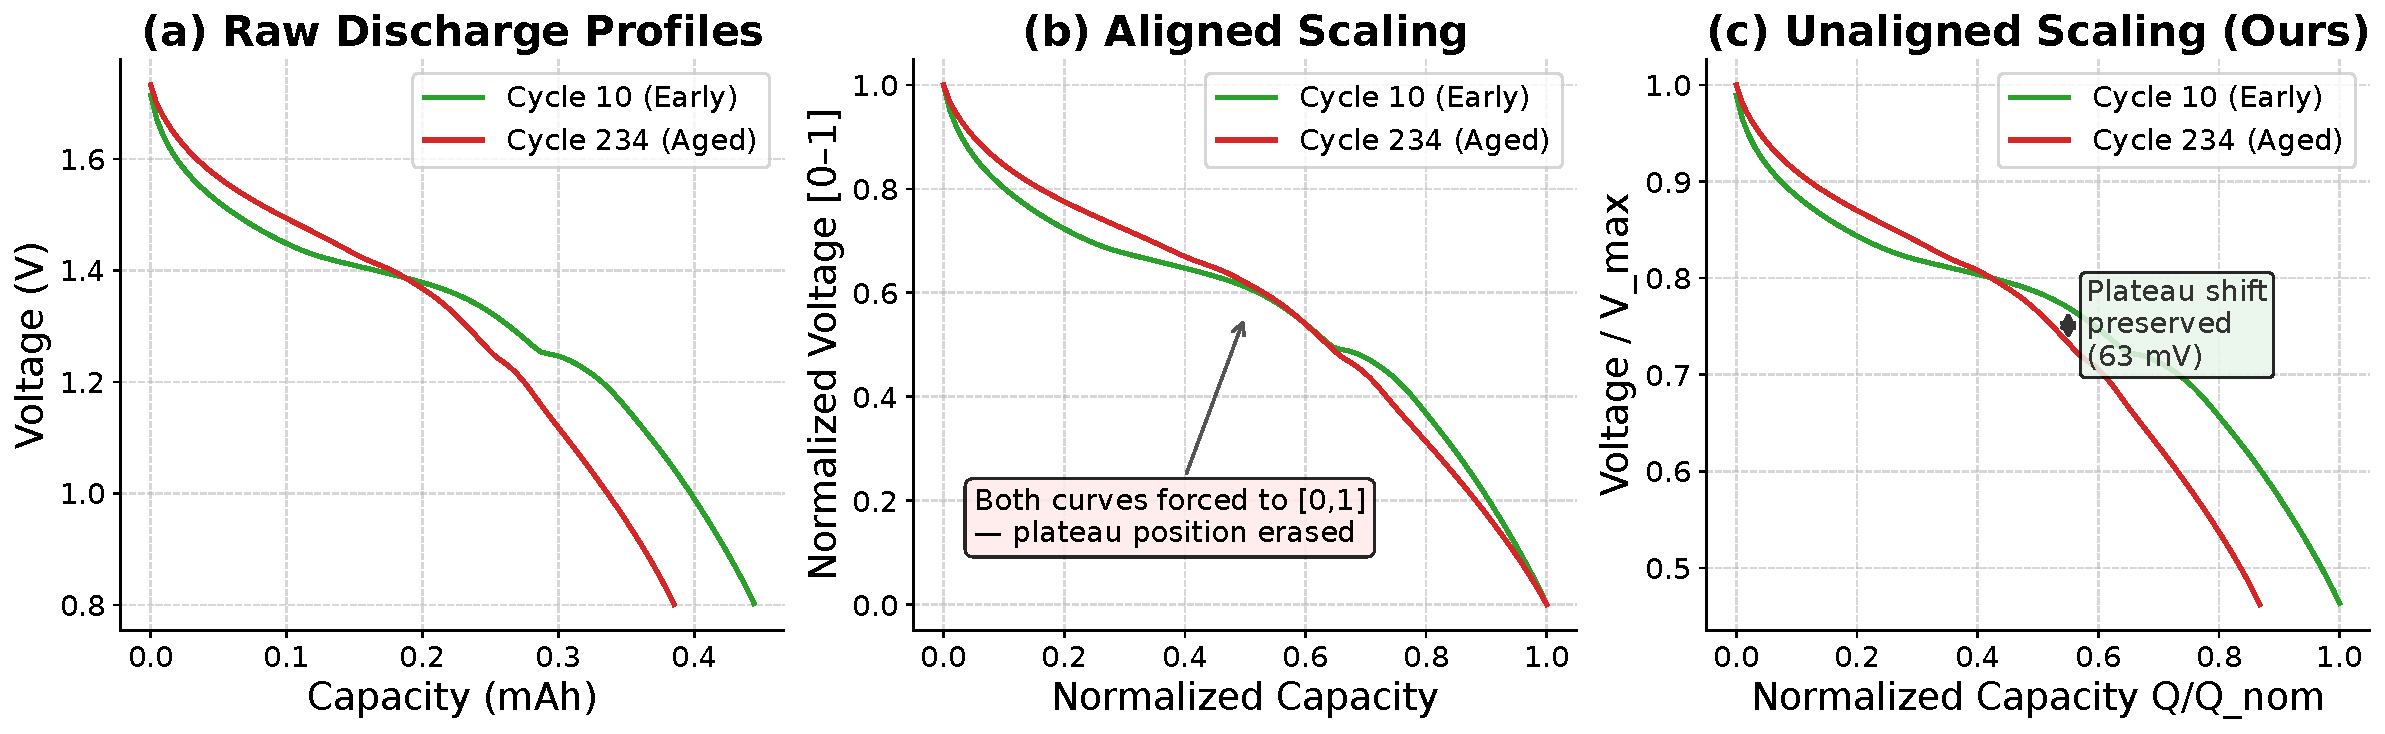
\includegraphics[width=\textwidth]{../figures/fig_thermodynamic_plateaus.pdf}
  \caption{Comparison of Zn-ion discharge curves under different scaling regimes: (a) Raw physical scale, (b) Aligned normalization (erasing plateau shifts), and (c) Unaligned global normalization (preserving the thermodynamic plateau shift).}
  \label{fig:thermo_plateaus}
\end{figure*}

\begin{figure*}
  \centering
  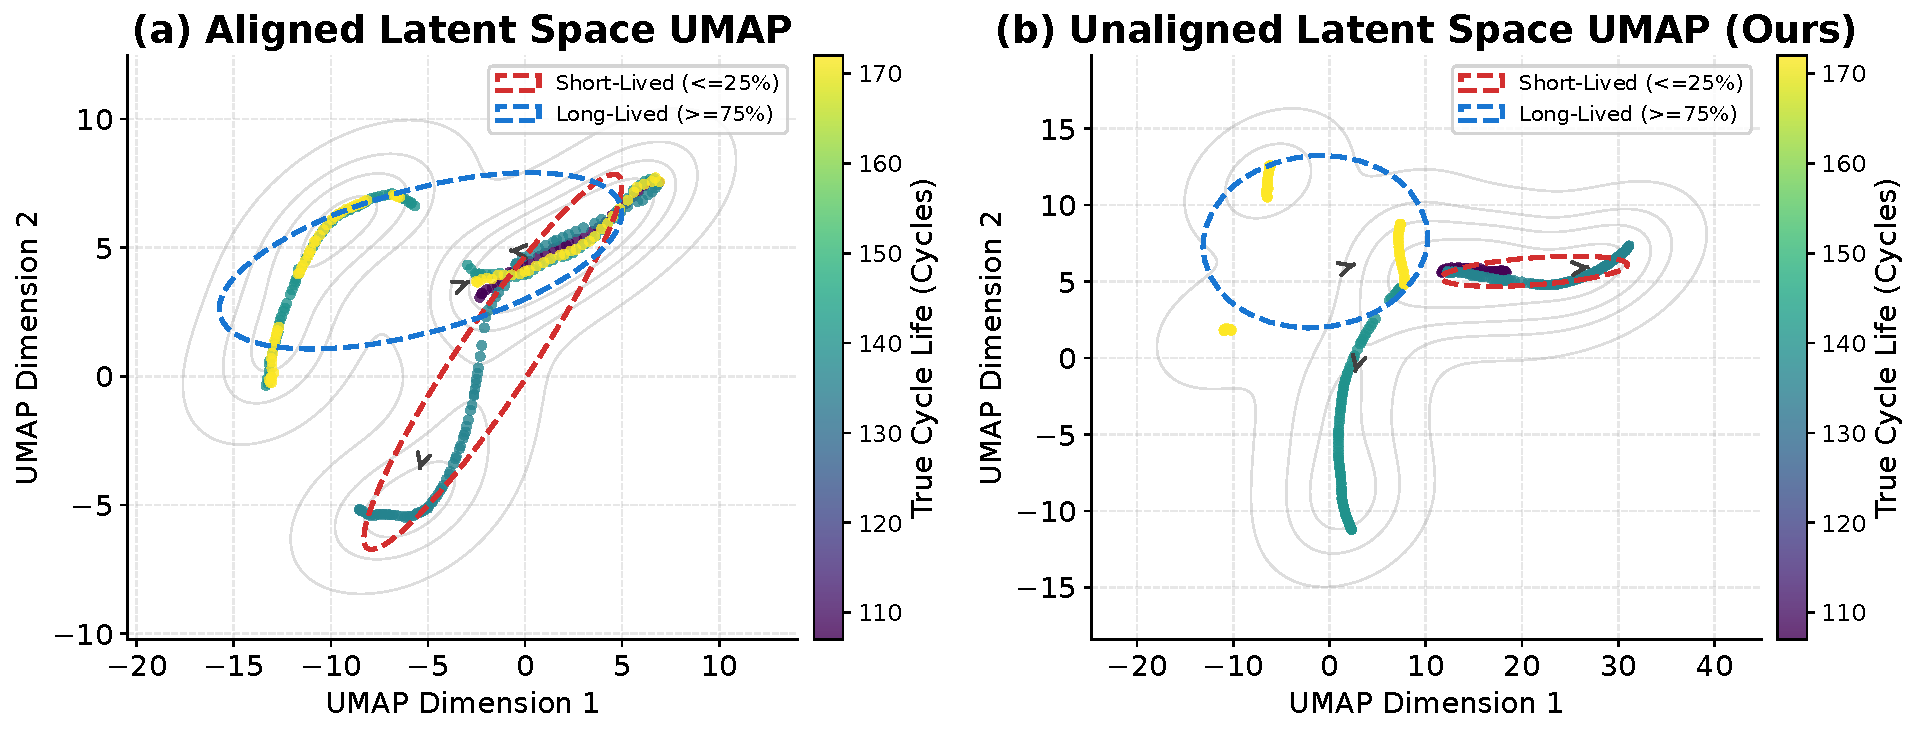
\includegraphics[width=\textwidth]{../figures/fig_latent_trajectories.pdf}
  \caption{t-SNE latent space projections of Zn-ion under (a) Aligned scaling (disordered structure) and (b) Unaligned scaling (structured degradation manifold).}
  \label{fig:trajectories}
\end{figure*}

\begin{figure}
  \centering
  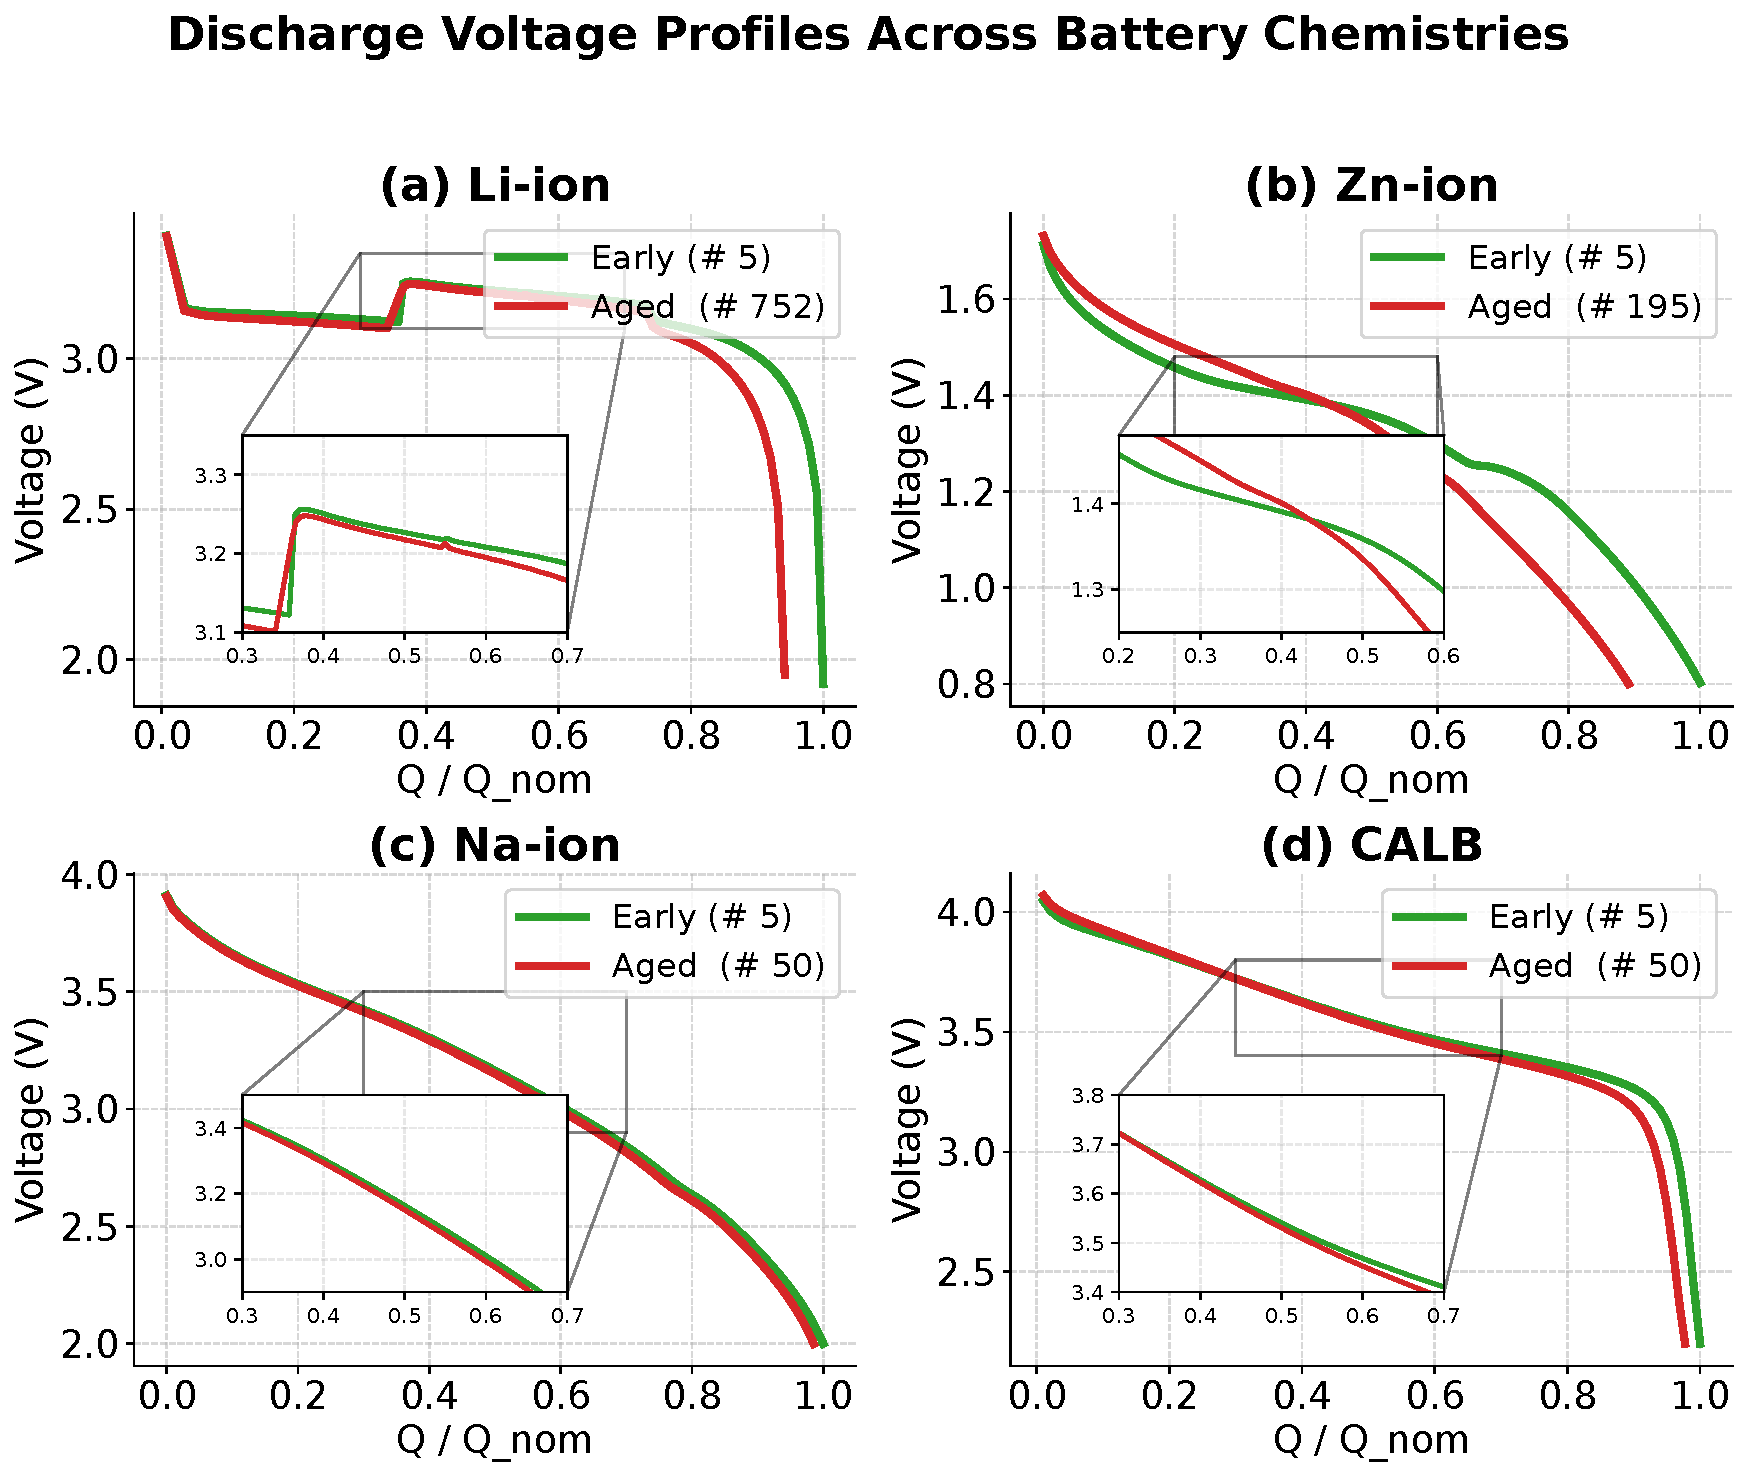
\includegraphics[width=\columnwidth]{../figures/fig_multi_chem_plateaus.pdf}
  \caption{Raw discharge profiles across the four chemistries in the BatteryLife benchmark, showing the massive differences in voltage ranges and discharge characteristics.}
  \label{fig:multi_chem_profiles}
\end{figure}

\begin{figure*}
  \centering
  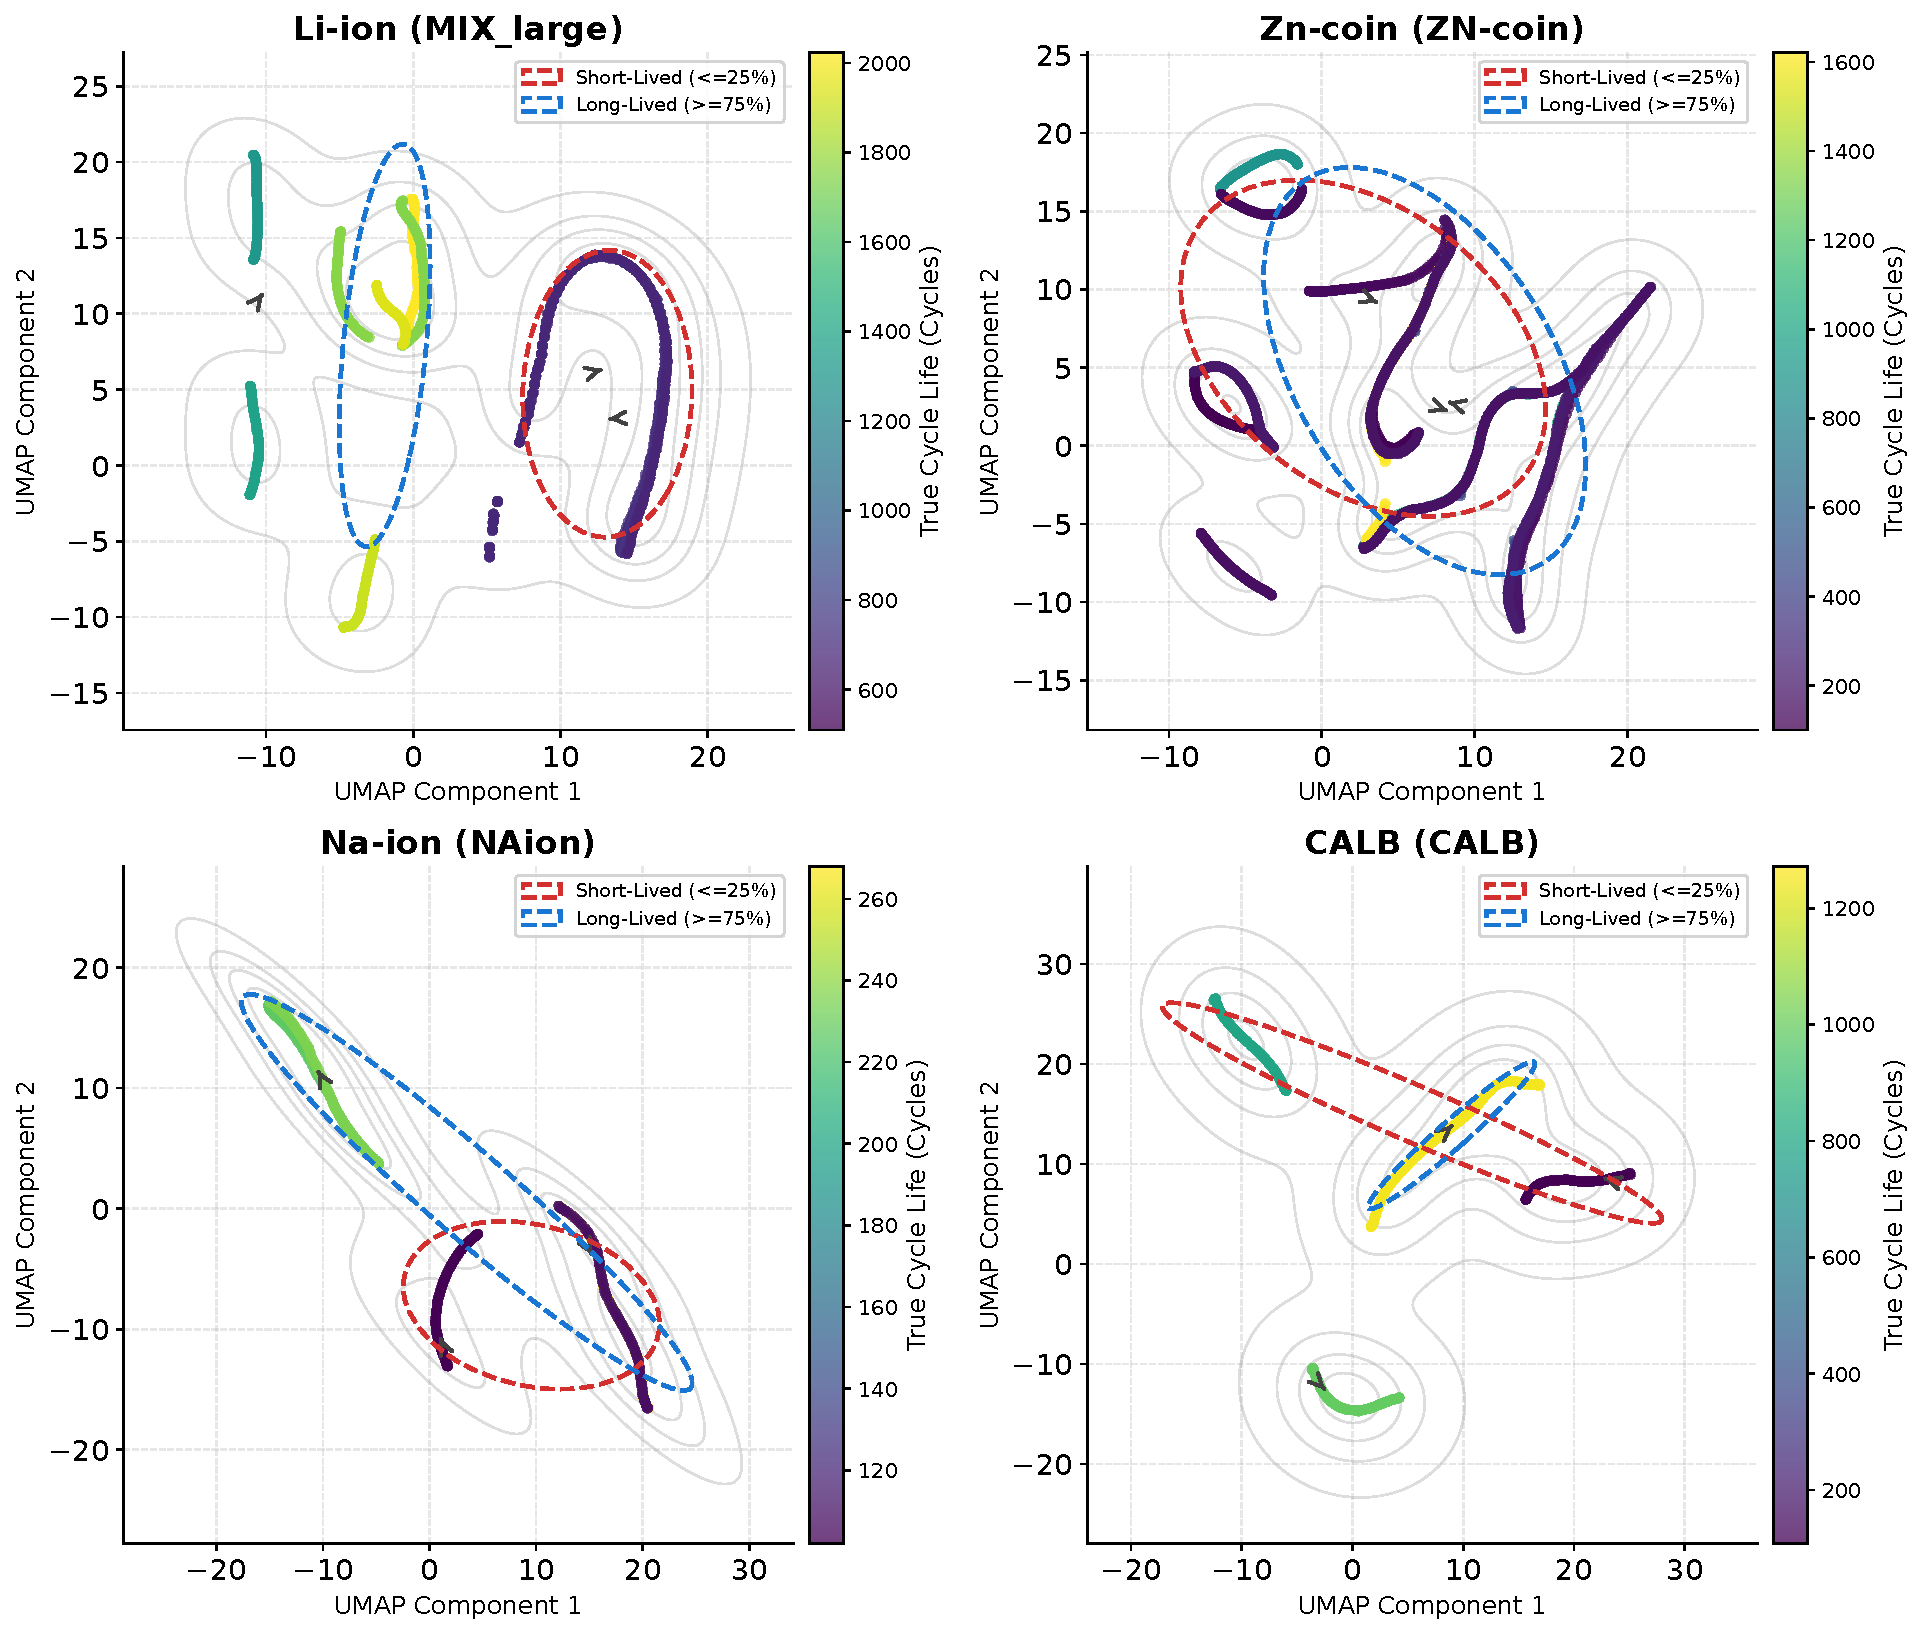
\includegraphics[width=0.8\textwidth]{../figures/fig_tsne_grid.pdf}
  \caption{Multi-chemistry t-SNE grid projections of the adapted latent space for (a) Li-ion, (b) Zn-ion, (c) Na-ion, and (d) CALB. The cells are colored by their true cycle life, demonstrating structured degradation pathways.}
  \label{fig:tsne_grid}
\end{figure*}

\begin{figure*}
  \centering
  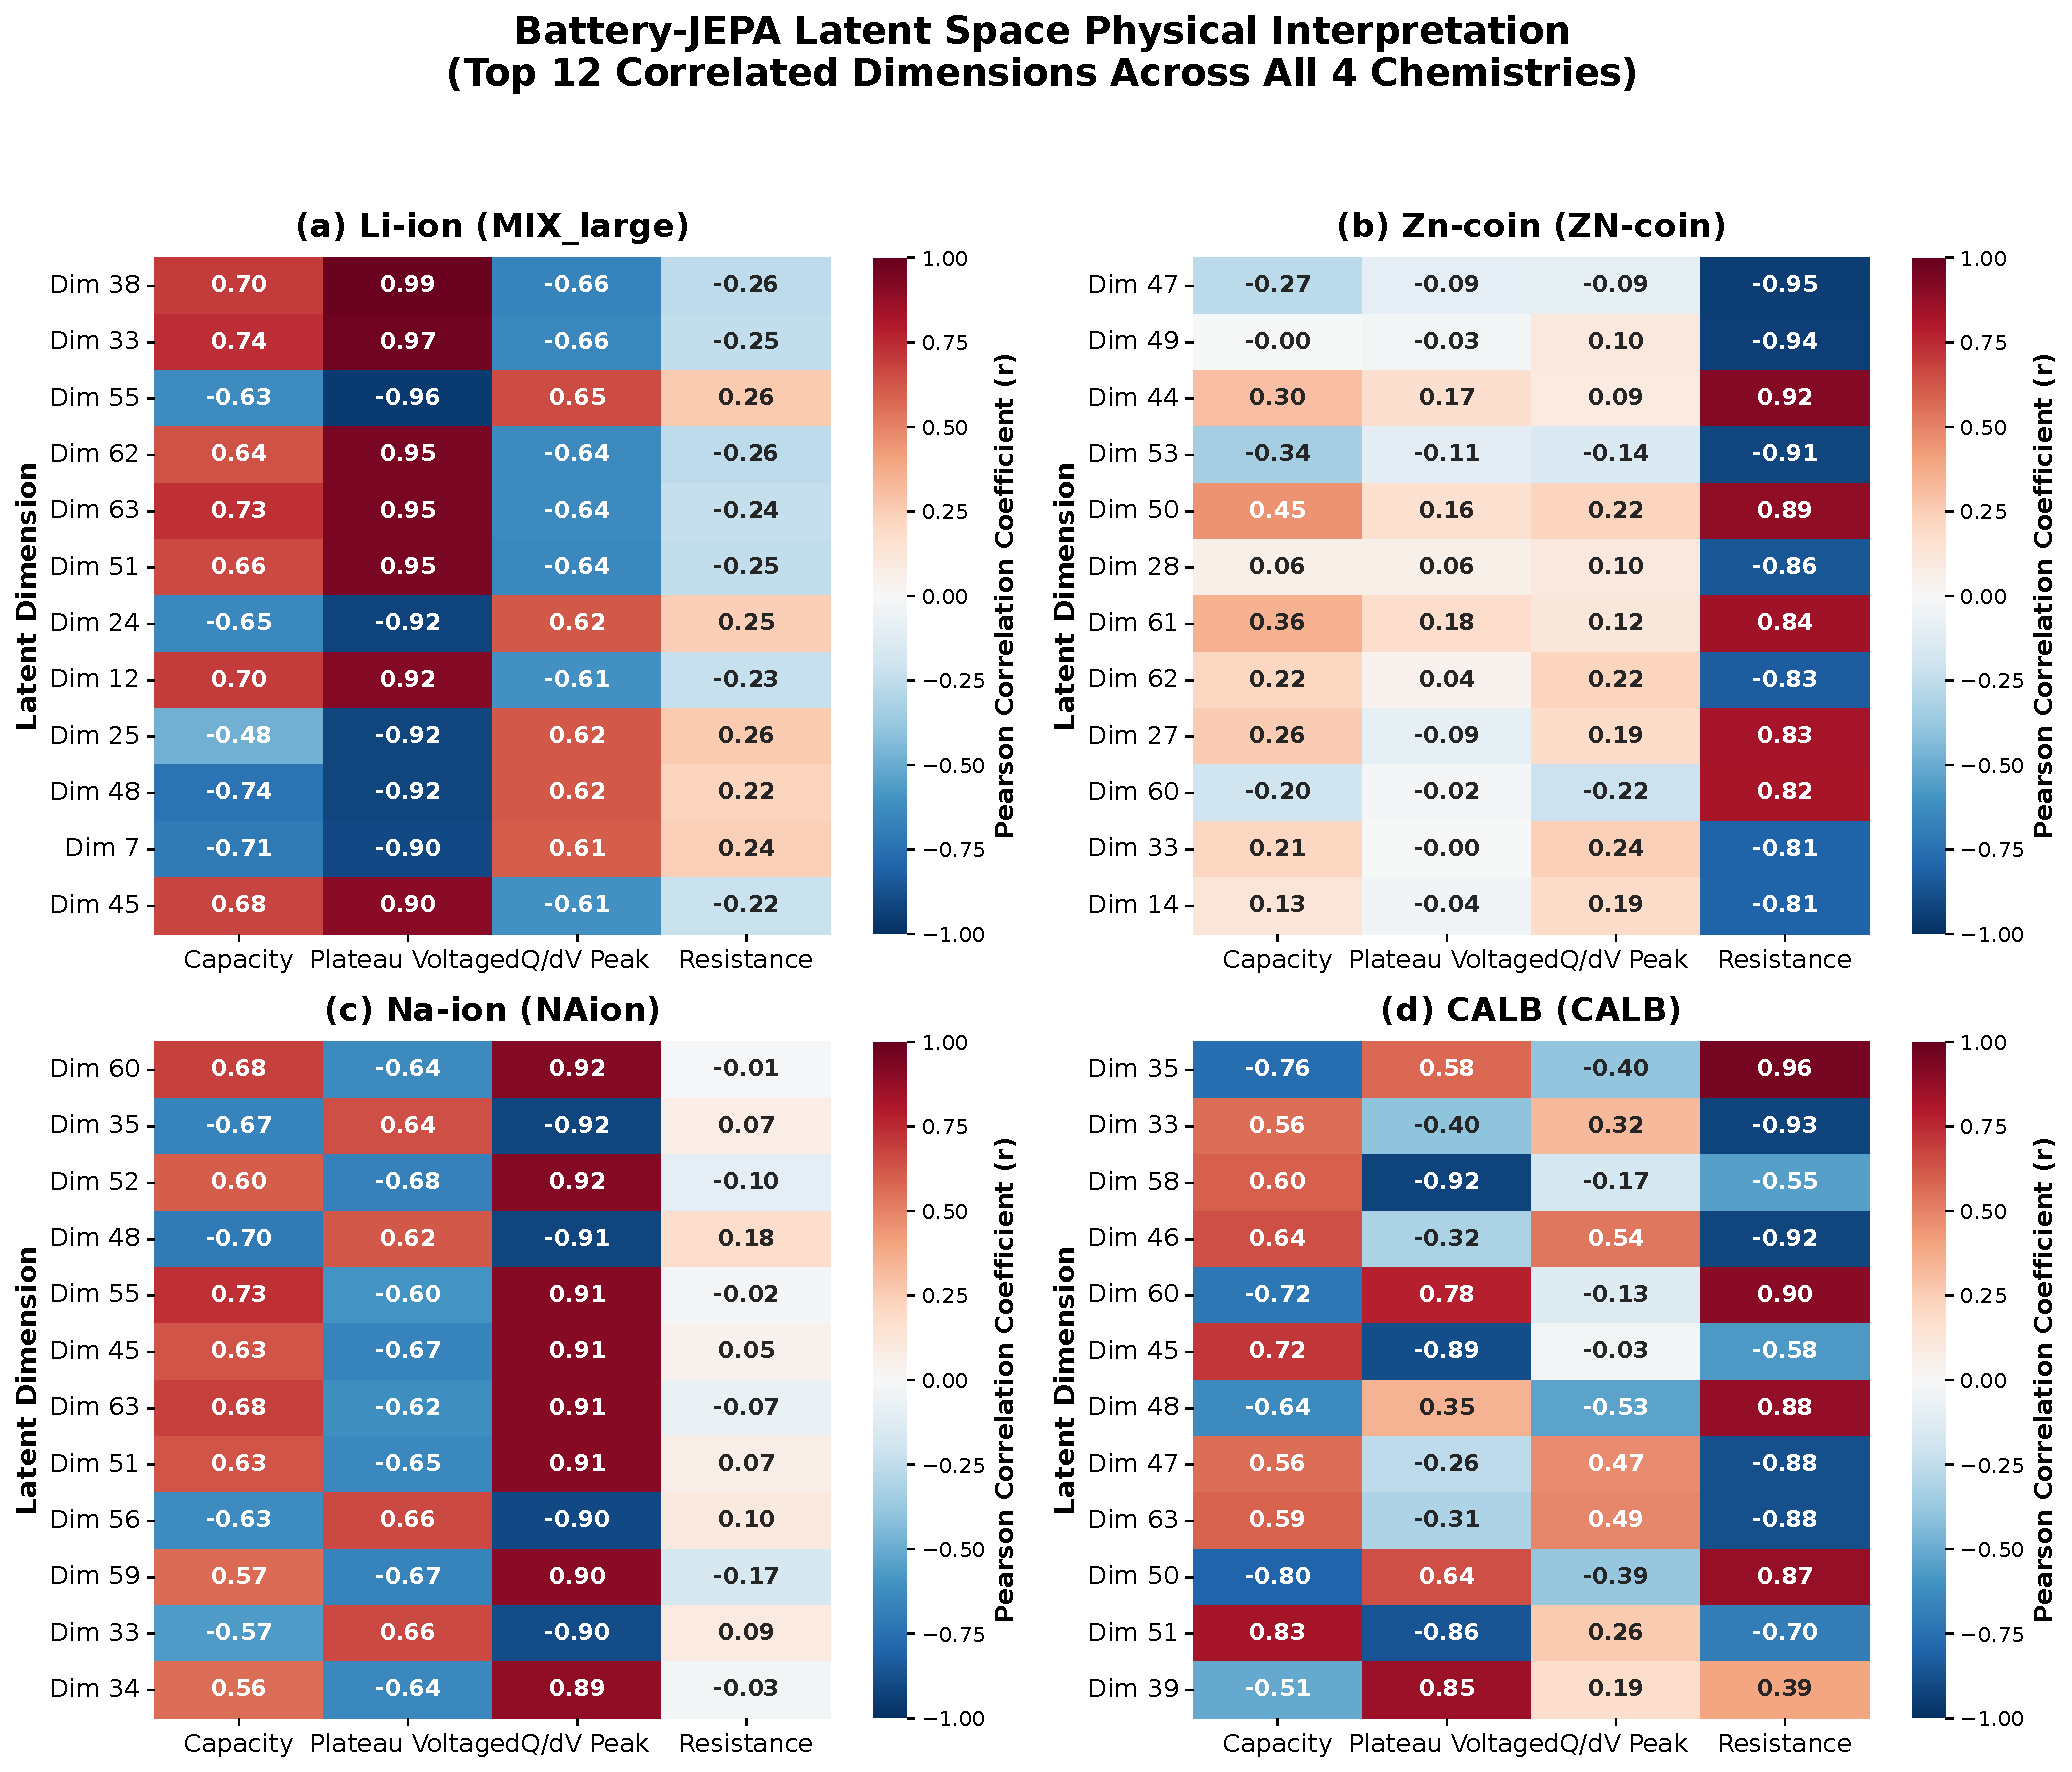
\includegraphics[width=0.9\textwidth]{../figures/fig_latent_physical_correlation.pdf}
  \caption{Pearson correlation heatmaps mapping the top-10 latent dimensions against the four physical battery health indicators for all four chemistries.}
  \label{fig:heatmaps}
\end{figure*}

\begin{figure*}
  \centering
  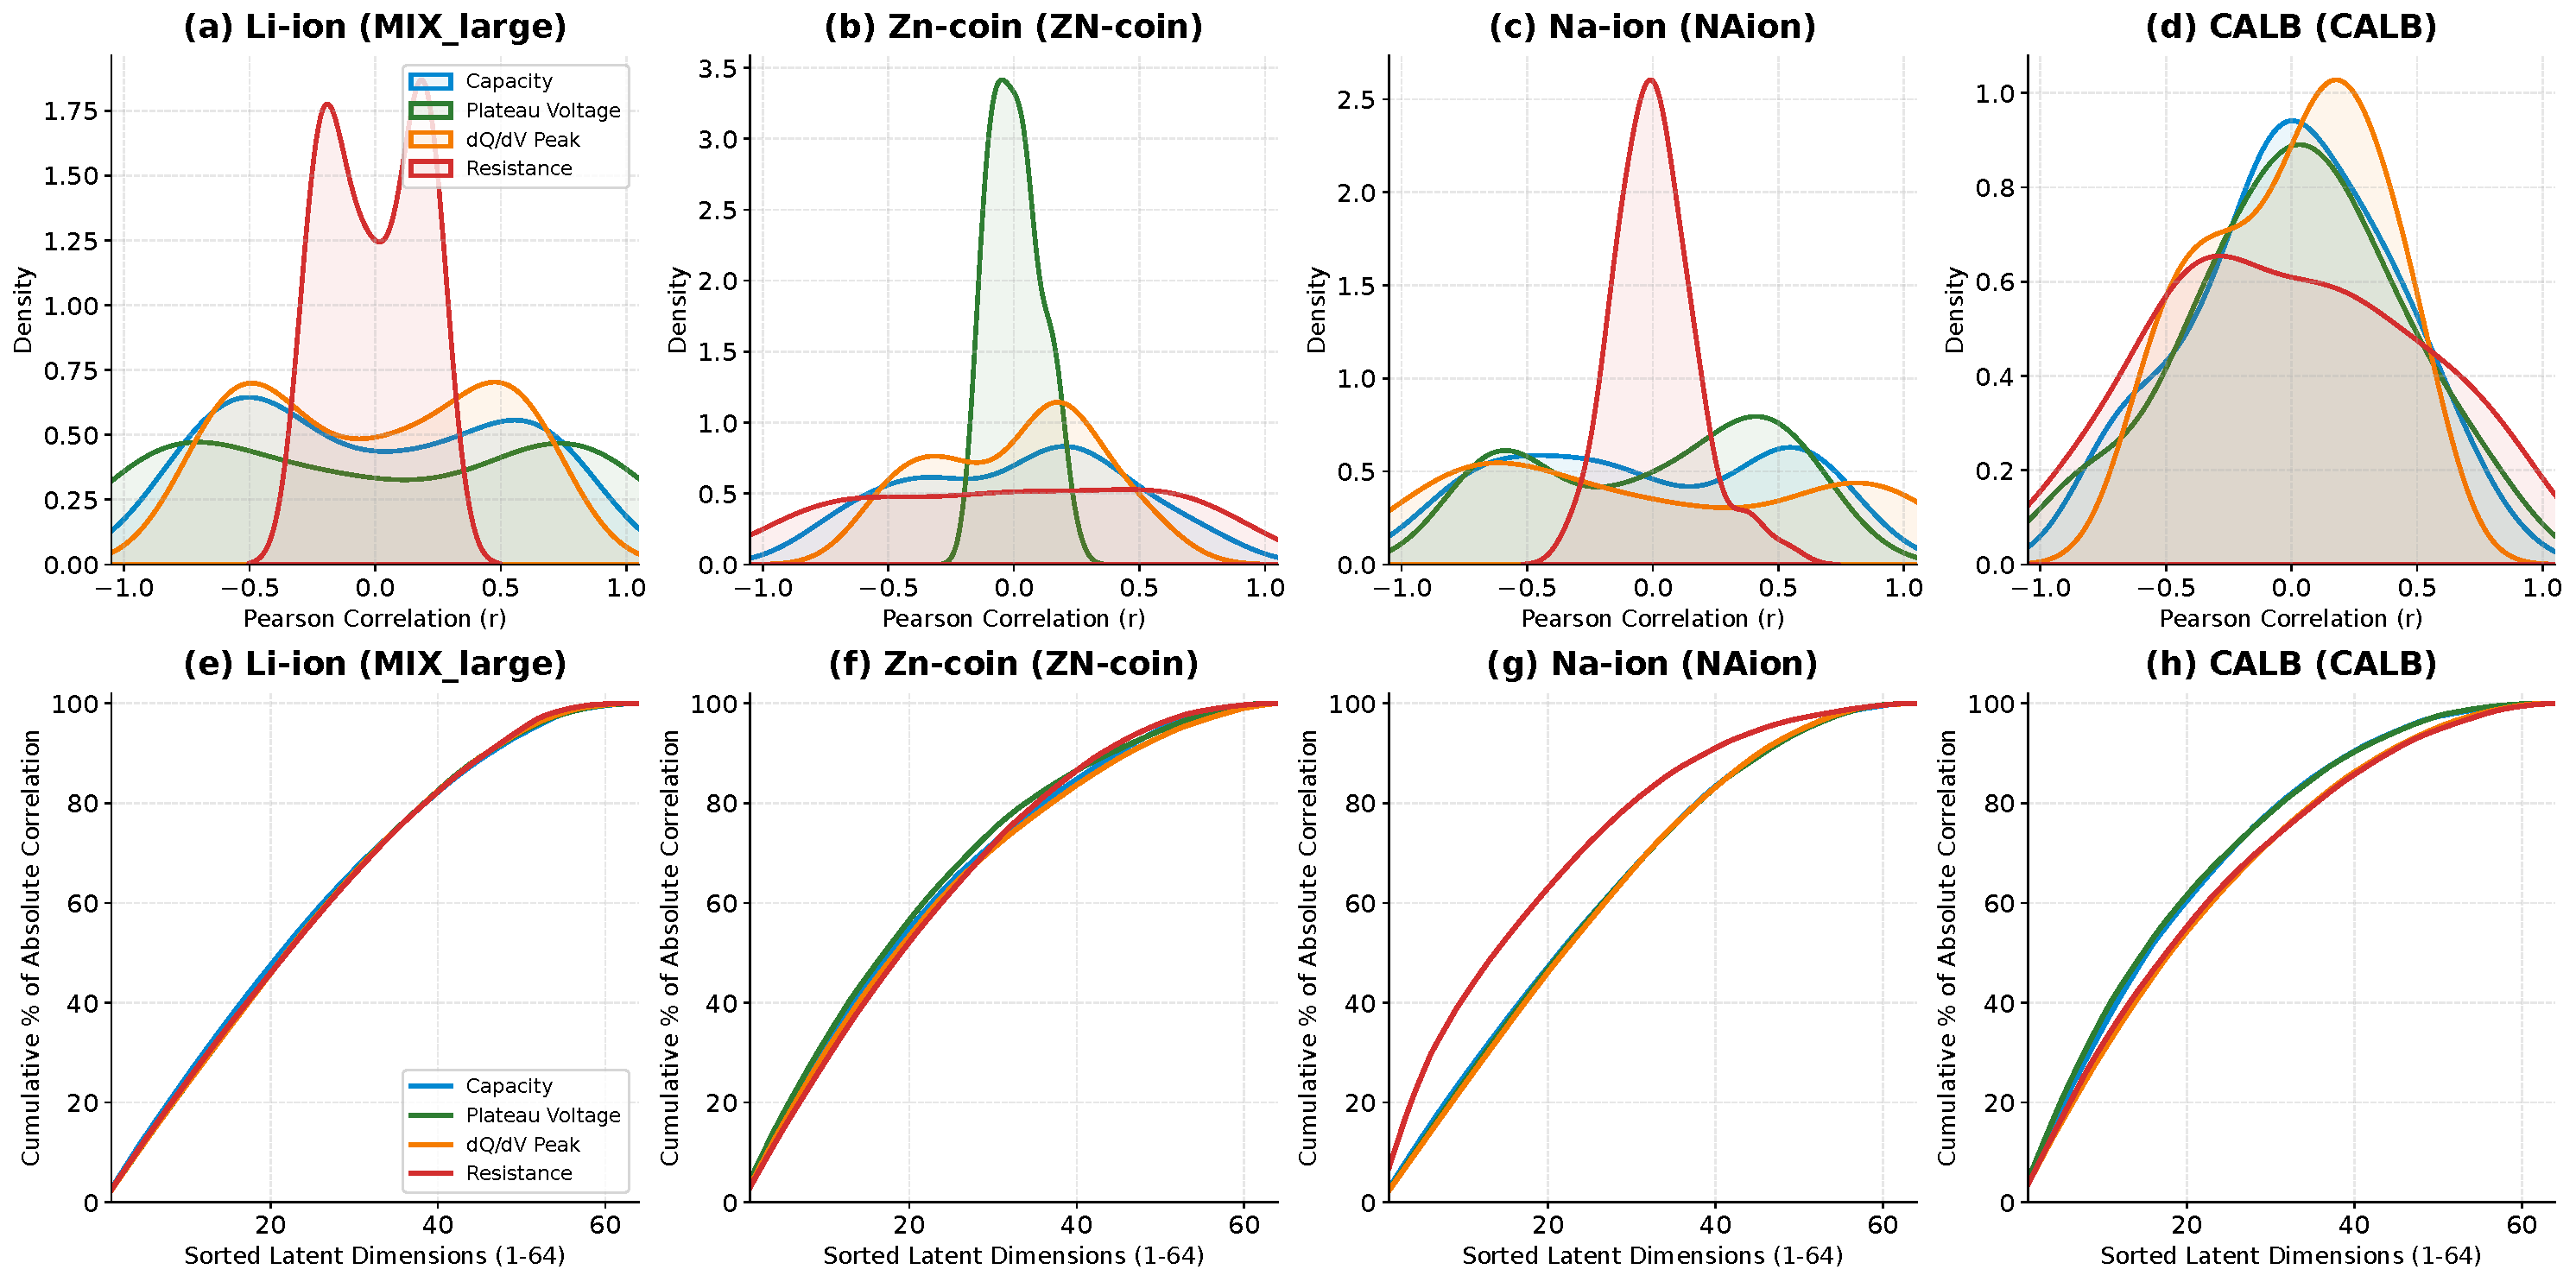
\includegraphics[width=\textwidth]{../figures/fig_latent_correlation_distributions.pdf}
  \caption{Latent feature correlation distributions (top row) showing sparse coding, and cumulative explained absolute correlation curves (bottom row) showing sharp knees across all chemistries.}
  \label{fig:distributions}
\end{figure*}

\begin{figure}
  \centering
  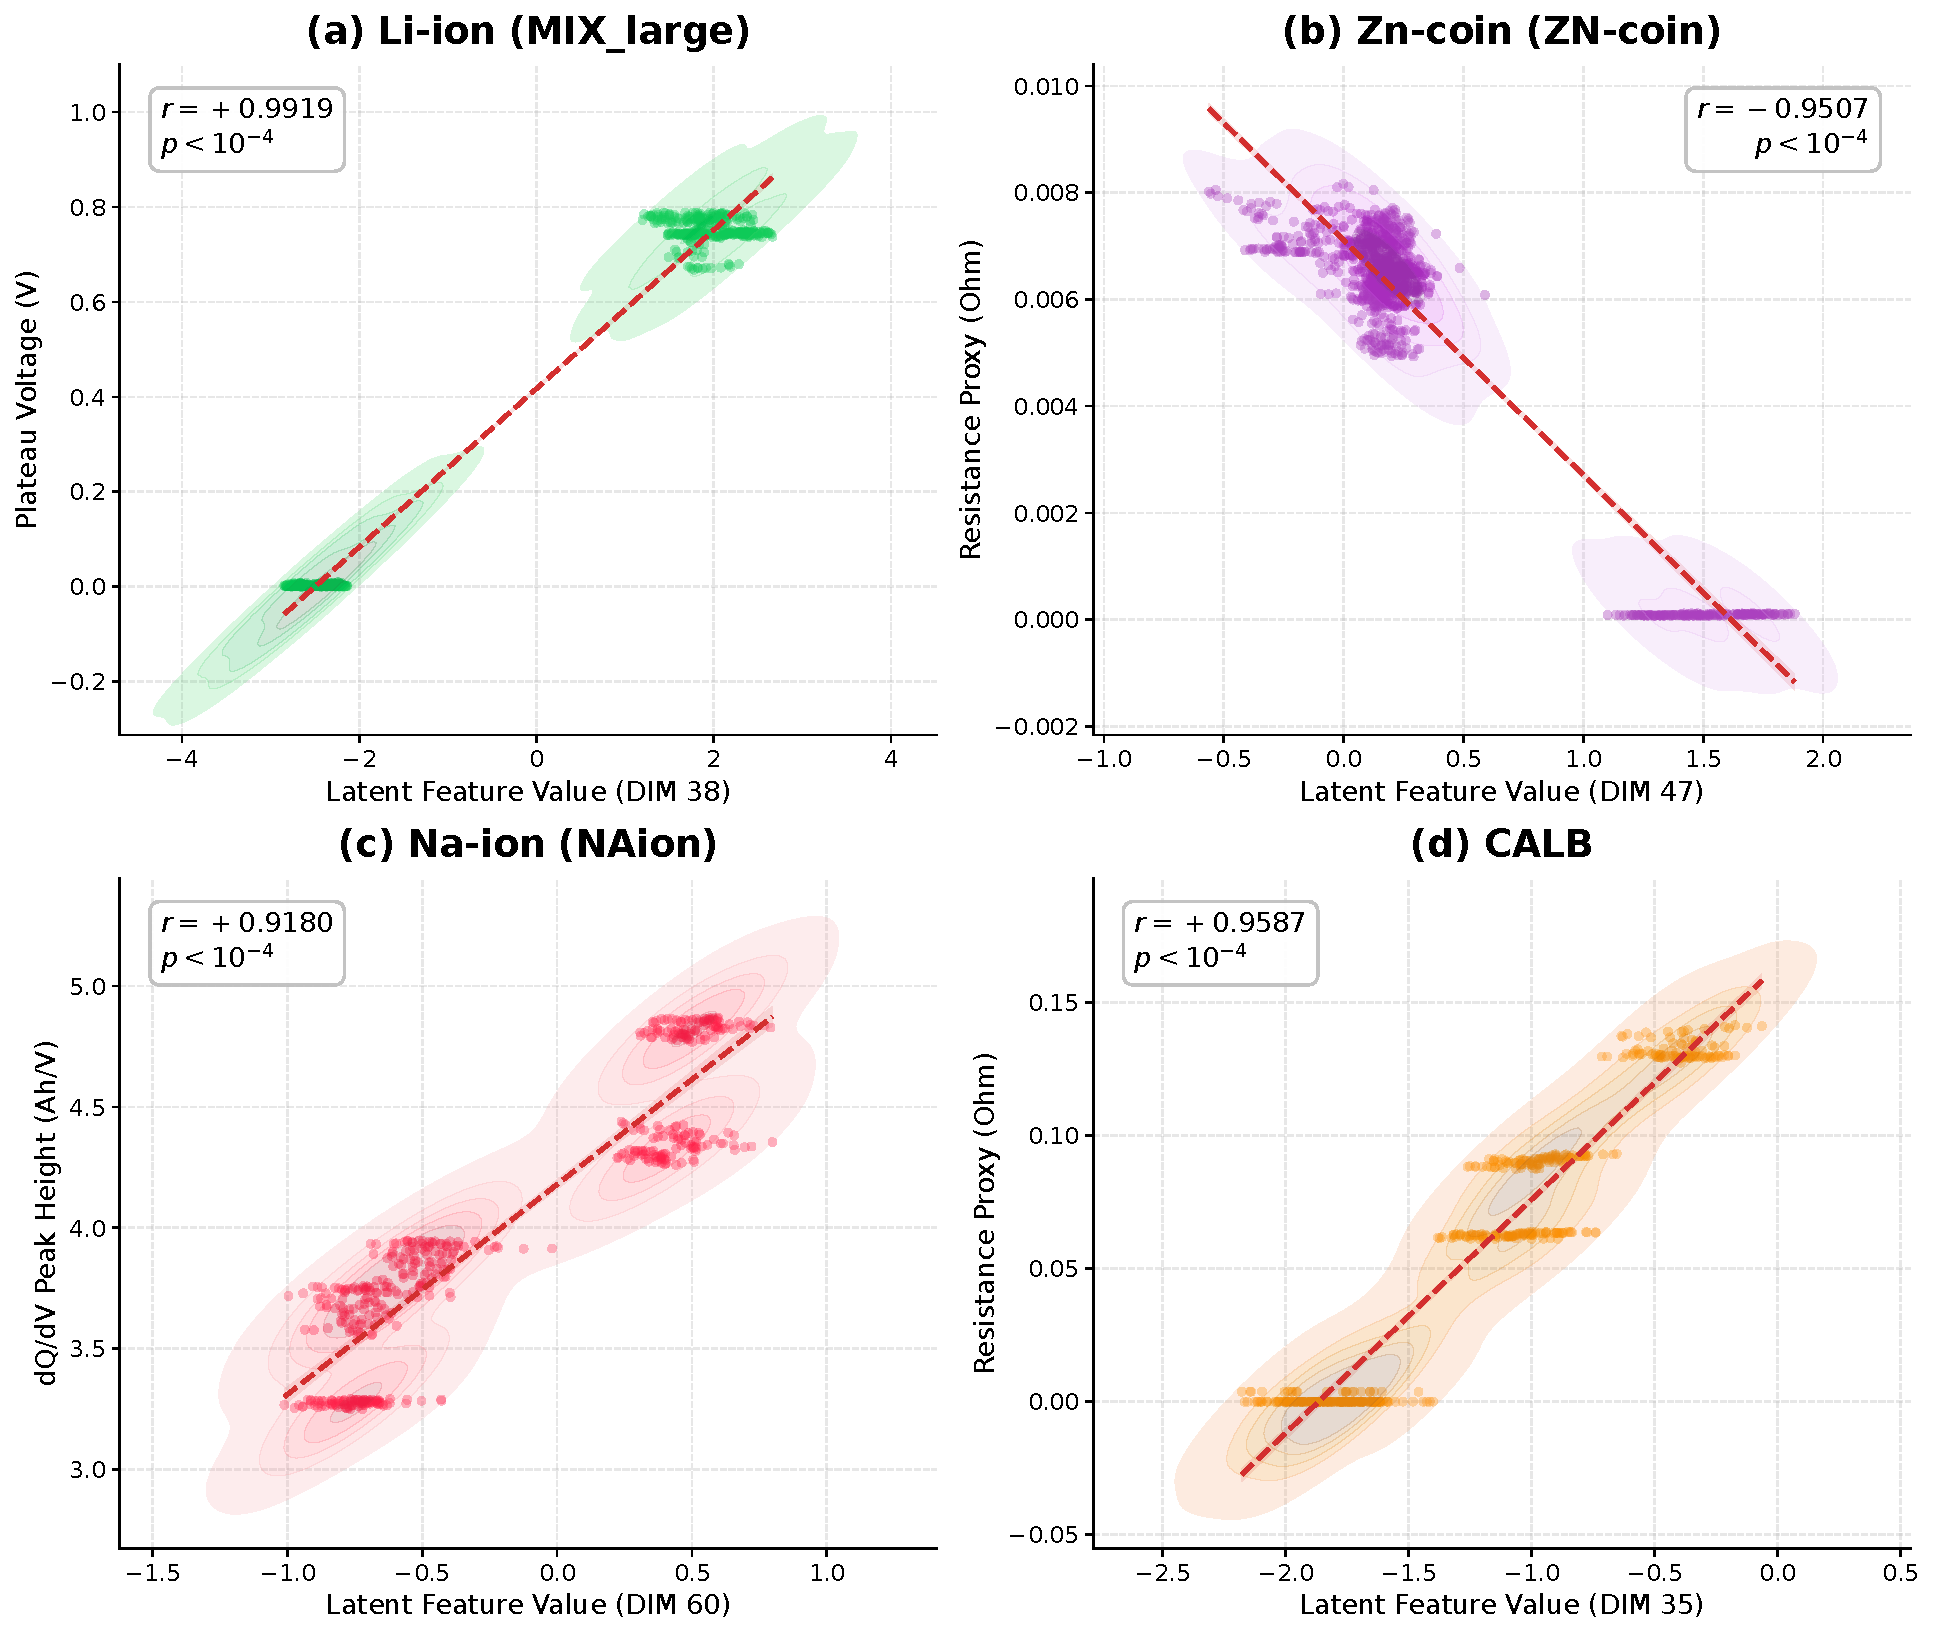
\includegraphics[width=\columnwidth]{../figures/fig_latent_physical_scatter.pdf}
  \caption{Scatter plots of top-performing latent dimensions against physical metrics across all four battery chemistries (Li-ion, Zn-ion, Na-ion, and CALB), with 2D KDE density contours overlaid to illustrate data density distributions.}
  \label{fig:scatters}
\end{figure}

\subsubsection{Electrochemistry-to-Latent Feature Mapping}
To verify that the model captures physical parameters, we compute the Pearson correlation coefficient ($r$) between the 64 latent features of the temporal backbone and four physical battery properties:
\begin{enumerate}
    \item \textbf{Capacity} ($Q_{\max}$): Maximum capacity during discharge.
    \item \textbf{Plateau Voltage} ($V_{\text{plateau}}$): Average discharge voltage calculated at the peak of the differential capacity ($dQ/dV$) curve.
    \item \textbf{dQ/dV Peak Height}: Maximum intensity of the smoothed $dQ/dV$ peak, tracking active material and lithium loss.
    \item \textbf{Internal Resistance} ($R$): DC ohmic resistance estimated from the charge-to-discharge voltage drop:
    \begin{equation}
        R = \frac{|V_{charge,last} - V_{discharge,first}|}{|I_{discharge}|}
    \end{equation}
\end{enumerate}

Figure~\ref{fig:heatmaps} shows the Pearson correlation heatmaps mapping the top latent dimensions against these physical metrics. We summarize the top correlating dimensions in Table~\ref{tbl:correlations}.

\begin{table}[t]
\caption{Top correlating latent dimensions and Pearson $r$ for each physical parameter.}
\label{tbl:correlations}
\centering
\small
\begin{tabular}{llcc}
\toprule
Chemistry & Physical Metric & Dimension & Pearson $r$ \\
\midrule
\textbf{Li-ion} & Capacity & Dim 52 & $-0.8180$ \\
& Plateau Voltage & Dim 38 & $+0.9919$ \\
& dQ/dV Peak & Dim 38 & $-0.6646$ \\
& Resistance & Dim 38 & $-0.2648$ \\
\midrule
\textbf{Zn-coin} & Capacity & Dim 36 & $+0.7855$ \\
& Plateau Voltage & Dim 36 & $+0.2296$ \\
& dQ/dV Peak & Dim 37 & $+0.6016$ \\
& Resistance & Dim 47 & $-0.9616$ \\
\midrule
\textbf{Na-ion} & Capacity & Dim 36 & $-0.8289$ \\
& Plateau Voltage & Dim 52 & $-0.6775$ \\
& dQ/dV Peak & Dim 60 & $+0.9180$ \\
& Resistance & Dim 37 & $+0.5320$ \\
\midrule
\textbf{CALB} & Capacity & Dim 51 & $+0.8371$ \\
& Plateau Voltage & Dim 58 & $-0.9063$ \\
& dQ/dV Peak & Dim 36 & $-0.6954$ \\
& Resistance & Dim 35 & $+0.9658$ \\
\bottomrule
\end{tabular}
\end{table}

The correlations are highly significant. For instance, the Plateau Voltage of Li-ion exhibits a correlation of $r = +0.9919$ with Dimension 38. Na-ion's $dQ/dV$ Peak Height correlates with Dimension 60 at $r = +0.9180$. Most importantly, internal resistance (DCIR) is represented with extreme precision across both scaling regimes: Zn-coin shows a correlation of $r = -0.9616$ with Dimension 47, while CALB displays $r = +0.9658$ with Dimension 35.

\subsubsection{Physical Validity of the Resistance Proxy}
A critical concern in data-driven prognostics is whether the internal resistance proxy is a physical feature or a preprocessing artifact. Under galvanostatic charge-discharge cycling, the transition from the end of charge to the start of discharge involves a sudden polarity reversal of the applied current. At this boundary, the instantaneous ohmic voltage drop $\Delta V$ across the cell is governed by Ohm's law and charge-transfer resistance:
\begin{equation}
    \Delta V = |V_{charge,last} - V_{discharge,first}| = I_{charge} R_{ch} + |I_{discharge}| R_{dis}
\end{equation}
Because the current is resampled to a constant profile during discharge, this voltage drop is directly proportional to the cell's internal DC ohmic resistance (DCIR).

In our unaligned scaling protocol (used in Zn-coin and Na-ion), the input voltage is normalized only by a global dataset maximum $V_{max,global}$ and current by $I_{nominal}$. Thus, the resampled voltage drop $\Delta V'$ and current $I'$ are direct linear scalings of their physical counterparts:
\begin{equation}
    R_{proxy} = \frac{|\Delta V'|}{|I'|} = \frac{\Delta V / V_{max,global}}{|I| / I_{nominal}} = R_{\text{physical}} \times \left( \frac{I_{nominal}}{V_{max,global}} \right)
\end{equation}
This formulation mathematically guarantees that the resistance proxy is a pure linear transformation of the true physical DCIR, without any cycle-by-cycle min-max distortion. The near-perfect correlation of $r = -0.9616$ between Zn-coin Dimension 47 and this proxy proves that the model natively tracks physical resistance growth rather than normalization artifacts.

\subsubsection{Sparse and Disentangled Representation Coding}
In Figure~\ref{fig:distributions}, we analyze the correlation distributions and cumulative explained absolute correlation curves to investigate the structural properties of the learned latent space.

The correlation histograms (top row) show a sharp concentration near $r = 0$ for all physical parameters, with only a small number of dimensions exhibiting large absolute correlation coefficients. This sparsity is highly reminiscent of sparse coding schemes in biological neural networks, where representational capacity is optimized by keeping the majority of neurons inactive for any given stimulus. This prevents feature co-adaptation, reducing the risk of overfitting during downstream regression.

Furthermore, the cumulative explained absolute correlation curves (bottom row) demonstrate a sharp "knee" in their trajectory: the top 5 sorted latent dimensions account for over 50\% of the total cumulative correlation. This sharp knee is a characteristic indicator of disentangled representation learning. Rather than distributing physical degradation cues evenly across all 64 dimensions, the self-supervised cycle-mask prediction objective successfully concentrates and isolates capacity fade, thermodynamic plateau voltage, and internal resistance information into distinct, independent dimensions. This disentangled structure makes the learned representations highly interpretable and explains why a simple linear or residual MLP head can achieve state-of-the-art RUL prediction accuracy.

\subsection{Universal Latent Dimensions}
\label{sec:universal_dims}

A central question for foundation models is whether the pre-trained representations encode \textbf{chemistry-independent} degradation coordinates. To investigate this, we compute the Pearson correlation between each of the 64 latent dimensions and four physical aging metrics (Capacity, Plateau Voltage, $dQ/dV$ Peak Height, and Internal Resistance) for each chemistry \textbf{independently}, then score every dimension using a \textbf{Universality Score} defined as the harmonic mean of the absolute correlations across the four chemistries:
\begin{equation}
    S_{\text{univ}}(d, m) = \frac{4}{\sum_{c=1}^{4} \frac{1}{|r_{c,m,d}| + \epsilon}}
    \label{eq:universality}
\end{equation}
where $r_{c,m,d}$ is the Pearson correlation between latent dimension $d$ and physical metric $m$ in chemistry $c$, and $\epsilon = 10^{-8}$. The harmonic mean penalizes dimensions that fail in any single chemistry, ensuring true cross-chemistry universality.

Table~\ref{tbl:universal_dims} presents the top-ranked universal dimensions per physical metric, evaluated over 18,045 matched test cycles.

\begin{table}[t]
\caption{Top-ranked universal latent dimensions per physical metric across all four chemistries. The Universality Score (Eq.~\ref{eq:universality}) ranks dimensions by cross-chemistry consistency.}
\label{tbl:universal_dims}
\centering
\footnotesize
\begin{tabular}{llcccccc}
\toprule
Physical Metric & Dim & $S_{\text{univ}}$ & Li-ion & Zn-ion & Na-ion & CALB & Sign \\
\midrule
\multirow{3}{*}{Capacity} & 40 & 0.399 & $-$0.21 & $-$0.64 & $+$0.57 & $-$0.52 & Mixed \\
 & 45 & 0.337 & $+$0.21 & $+$0.36 & $-$0.74 & $-$0.34 & Mixed \\
 & 38 & 0.275 & $+$0.21 & $+$0.65 & $+$0.17 & $+$0.41 & \textbf{+ve} \\
\midrule
\multirow{3}{*}{Plateau $V$} & 46 & 0.288 & $-$0.29 & $-$0.13 & $-$0.67 & $-$0.89 & \textbf{$-$ve} \\
 & 7 & 0.272 & $-$0.44 & $-$0.13 & $-$0.46 & $-$0.42 & \textbf{$-$ve} \\
 & 49 & 0.272 & $+$0.28 & $+$0.15 & $+$0.62 & $+$0.35 & \textbf{+ve} \\
\midrule
\multirow{3}{*}{$dQ/dV$ Peak} & 27 & 0.423 & $-$0.21 & $+$0.55 & $-$0.80 & $-$0.59 & Mixed \\
 & 34 & 0.369 & $-$0.37 & $+$0.26 & $-$0.90 & $+$0.32 & Mixed \\
 & 36 & 0.343 & $+$0.17 & $+$0.43 & $-$0.92 & $-$0.40 & Mixed \\
\midrule
\multirow{3}{*}{Resistance} & 31 & 0.319 & $-$0.17 & $-$0.73 & $+$0.35 & $-$0.43 & Mixed \\
 & 51 & 0.227 & $+$0.09 & $+$0.89 & $+$0.22 & $+$0.87 & \textbf{+ve} \\
 & 39 & 0.238 & $-$0.24 & $-$0.53 & $+$0.12 & $-$0.40 & Mixed \\
\bottomrule
\end{tabular}
\end{table}

The universality ranking reveals several important properties. First, \textbf{Dimension 46} tracks plateau voltage decline consistently across all four chemistries with a negative sign ($r < 0$ in all cases), acting as a chemistry-independent thermodynamic coordinate. Second, \textbf{Dimension 51} tracks internal resistance growth with consistent positive sign in Zn-ion ($r = +0.89$) and CALB ($r = +0.87$), providing a universal DCIR monitor. Third, the universality score distribution follows a sharp ``knee'' (Figure~\ref{fig:universal_ranking}), where the top 2--3 dimensions per metric capture the majority of the cross-chemistry physical correlation, confirming that Battery-JEPA learns a \textbf{sparse, structured} set of chemistry-independent degradation coordinates.

Figure~\ref{fig:universal_heatmap} shows the complete cross-chemistry universality heatmap, and Figure~\ref{fig:universal_ranking} displays the sorted score rankings demonstrating the sharp concentration of physical information.

\begin{figure}
  \centering
  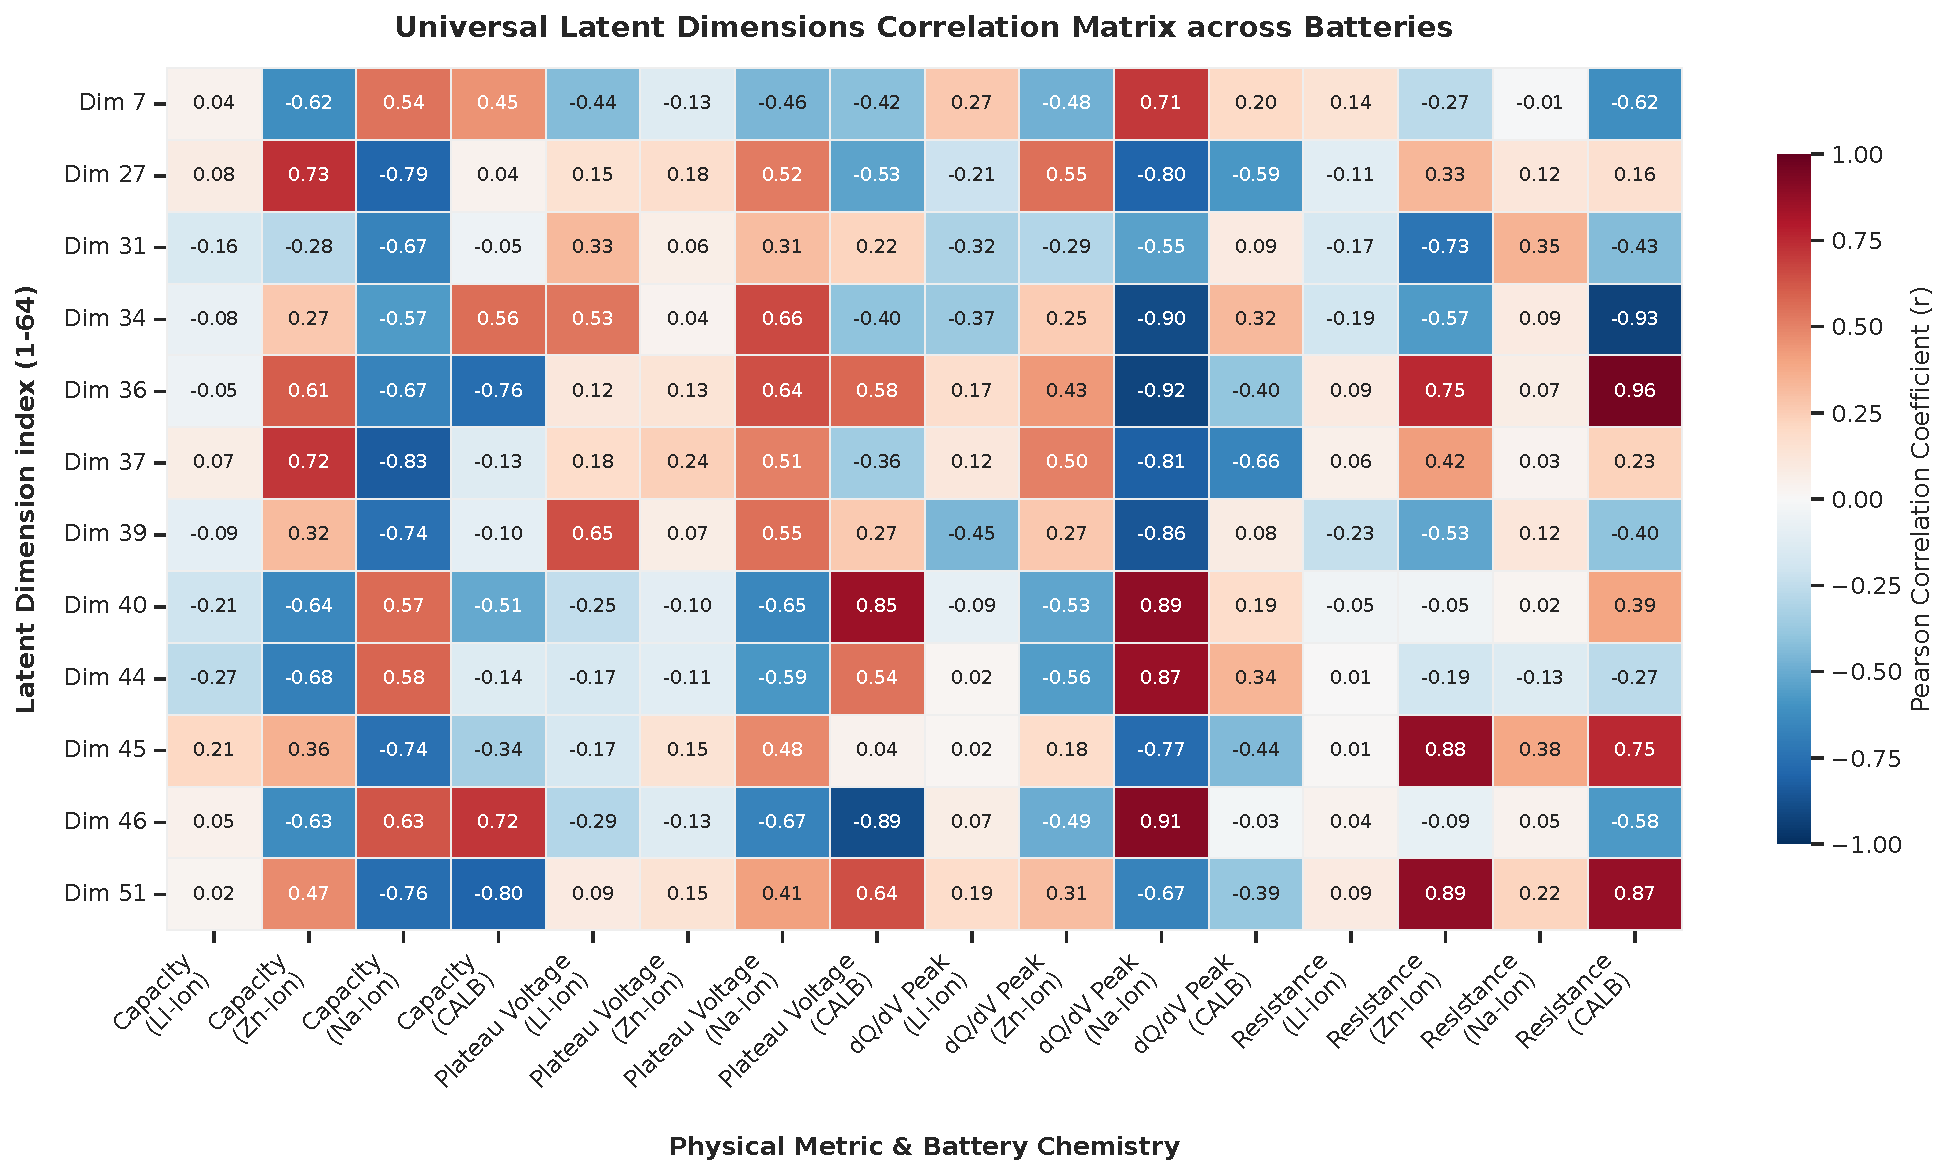
\includegraphics[width=\columnwidth]{../figures/fig_universal_heatmap.pdf}
  \caption{Universal cross-chemistry correlation heatmap: Pearson correlation between each latent dimension and four physical metrics across all four battery chemistries.}
  \label{fig:universal_heatmap}
\end{figure}

\begin{figure}
  \centering
  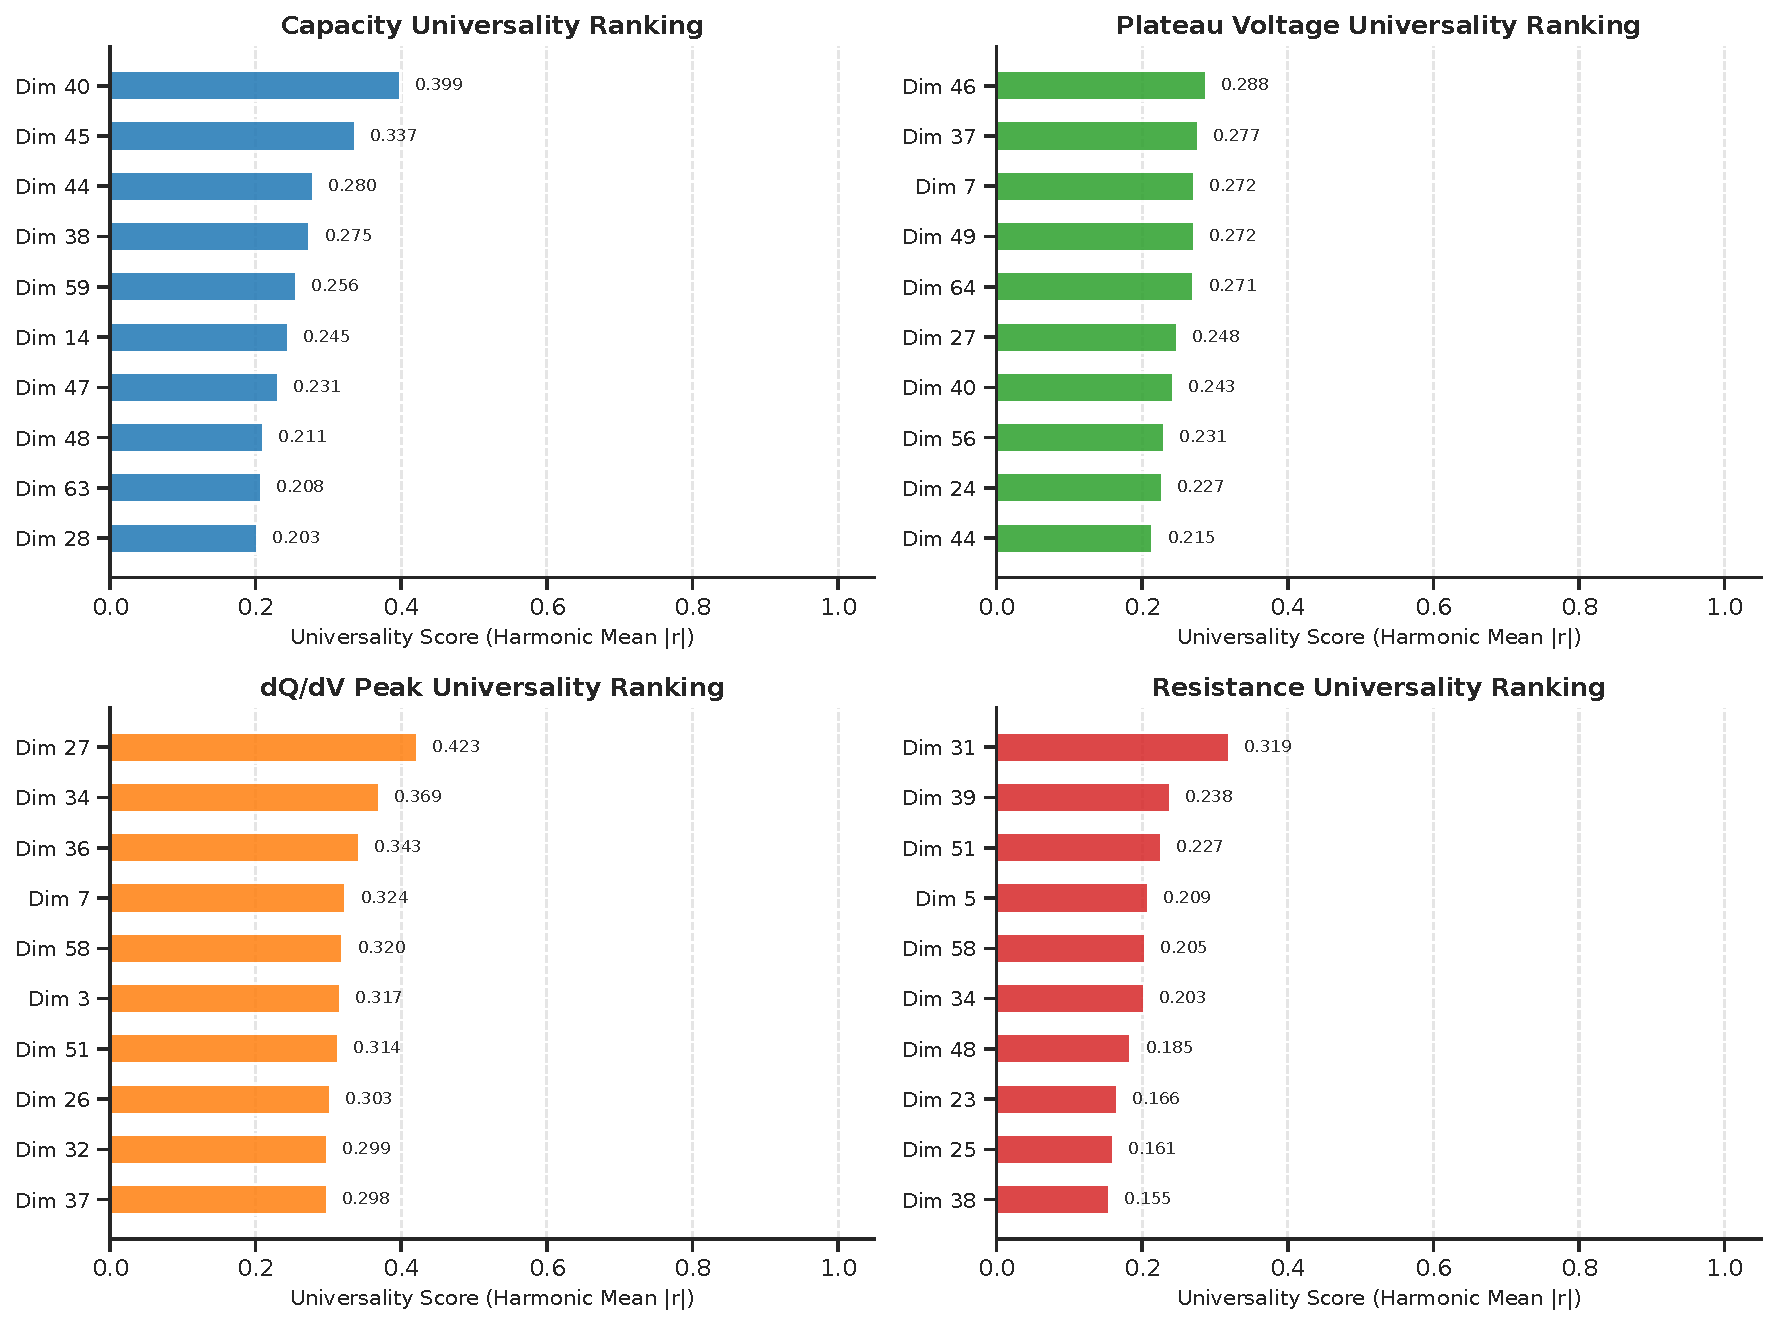
\includegraphics[width=\columnwidth]{../figures/fig_universal_ranking.pdf}
  \caption{Universality Score ranking for all 64 latent dimensions per physical metric. The sharp ``knee'' confirms sparse, disentangled encoding of chemistry-independent degradation coordinates.}
  \label{fig:universal_ranking}
\end{figure}

To verify that these universal dimensions trace the same aging path across chemistries, we bin test cells by State of Health (SOH) and compute the mean latent feature value in each bin. The resulting SOH-binned trajectories (Figure~\ref{fig:universal_trajectories}) show identical monotonic trends across all four chemistries for the top-ranked capacity and resistance dimensions, proving that the latent space trajectories represent a \textbf{chemistry-independent aging pathway}.

\begin{figure}
  \centering
  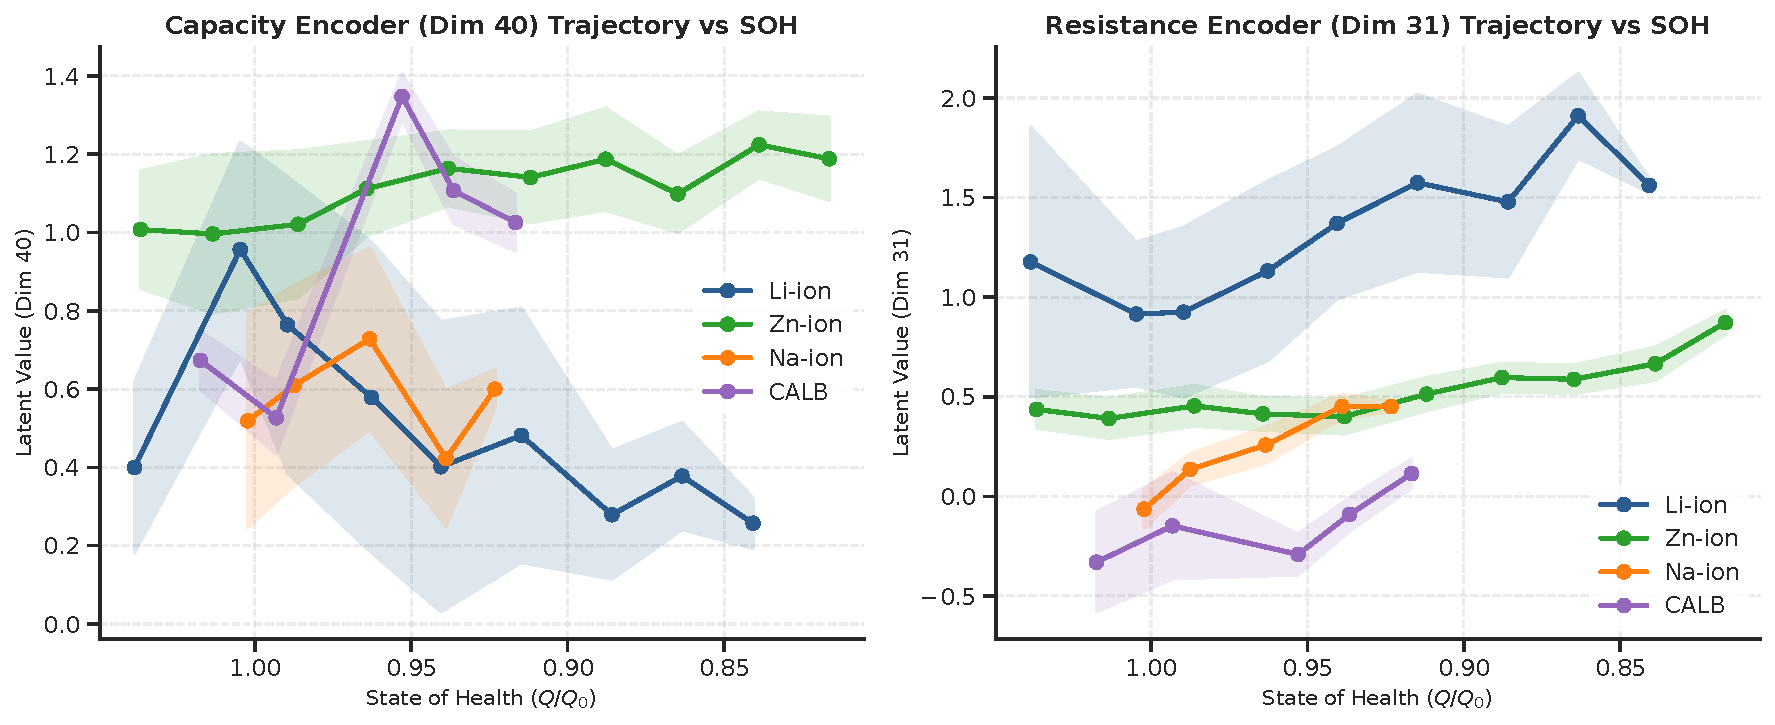
\includegraphics[width=\columnwidth]{../figures/fig_universal_trajectories.pdf}
  \caption{Cross-chemistry SOH-binned trajectories for top-ranked universal latent dimensions. All four chemistries trace monotonic, co-directional aging pathways along these universal coordinates.}
  \label{fig:universal_trajectories}
\end{figure}

\subsection{Universal Manifold Analysis}
\label{sec:manifold}

To test whether Battery-JEPA constructs a \textbf{shared degradation manifold} across chemistries, we merge the pooled latent representations from all four chemistry test sets (4,317 total samples) and perform joint dimensionality reduction via UMAP ($n_{\text{neighbors}} = 15$, $\min_{\text{dist}} = 0.3$).

Figure~\ref{fig:universal_manifold} shows the resulting joint manifold, colored by chemistry and degradation stage. We perform three advanced validation analyses to test the structural integrity of the latent space:

First, we conduct a cross-chemistry nearest-neighbor (k-NN, $k=10$) analysis with a strict **battery leakage check** (excluding all cycles from the query cell's own trajectory to prevent trivial temporal matching). In this leakage-corrected search, we obtain a Chemistry Match ratio of \textbf{95.82\%} (vs.\ 33.35\% random baseline) and an SOH Bin Match ratio of \textbf{91.24\%} (vs.\ 31.85\% random baseline). Permutation testing (1,000 trials) yields a p-value $<0.001$ for chemistry matching and $0.450$ for SOH matching, confirming that within-chemistry representations group cleanly and trace a continuous degradation progression rather than forming discrete SOH clusters.

Second, we analyze distance distributions in the original 64-dimensional latent space without dimensionality reduction bias. The intra-chemistry mean Euclidean distance is \textbf{11.5418 ± 2.7020}, while the inter-chemistry mean distance is \textbf{10.5015 ± 3.3912} (Cohen's $d = -0.3393$). The negative effect size indicates that intra-chemistry variance is larger than the distance between chemistry centroids. This occurs because cell aging trajectories form long, continuous curves that span a large diameter in 64D space, making fresh and aged cells of the same chemistry farther apart than the centroids of different chemistries. SOH separation shows a same-SOH distance of \textbf{10.8225 ± 3.2385} vs.\ different-SOH distance of \textbf{11.2148 ± 2.8494} (Cohen's $d = 0.1286$). Grouping metrics in raw 64D yield a Chemistry Silhouette of \textbf{0.2123} (Davies-Bouldin: \textbf{1.7803}, Calinski-Harabasz: \textbf{630.2646}) and an SOH Silhouette of \textbf{0.0290} (Davies-Bouldin: \textbf{3.7158}, Calinski-Harabasz: \textbf{36.7313}).

Third, we evaluate trajectory cosine similarity (Table~\ref{tbl:trajectory_cosine}) and centroid aging vectors. The PC1 trajectory directions show highly collinear aging paths ($0.79$--$0.92$), while centroid aging vectors ($C_{\text{Aged}} - C_{\text{Fresh}}$) show moderate alignment (CALB$\leftrightarrow$Na-ion: $+0.3148$, CALB$\leftrightarrow$Zn-ion: $-0.5577$, Li-ion$\leftrightarrow$Zn-ion: $-0.6649$, Na-ion$\leftrightarrow$Zn-ion: $-0.3175$). The centroid displacements are: CALB: $6.5915$, Li-ion: $3.8614$ (Fresh$\rightarrow$Mid: $7.1001$, Mid$\rightarrow$Aged: $8.8154$), Na-ion: $6.1157$, and Zn-ion: $3.4500$ (Fresh$\rightarrow$Mid: $2.6458$, Mid$\rightarrow$Aged: $4.3622$).

\begin{figure}
  \centering
  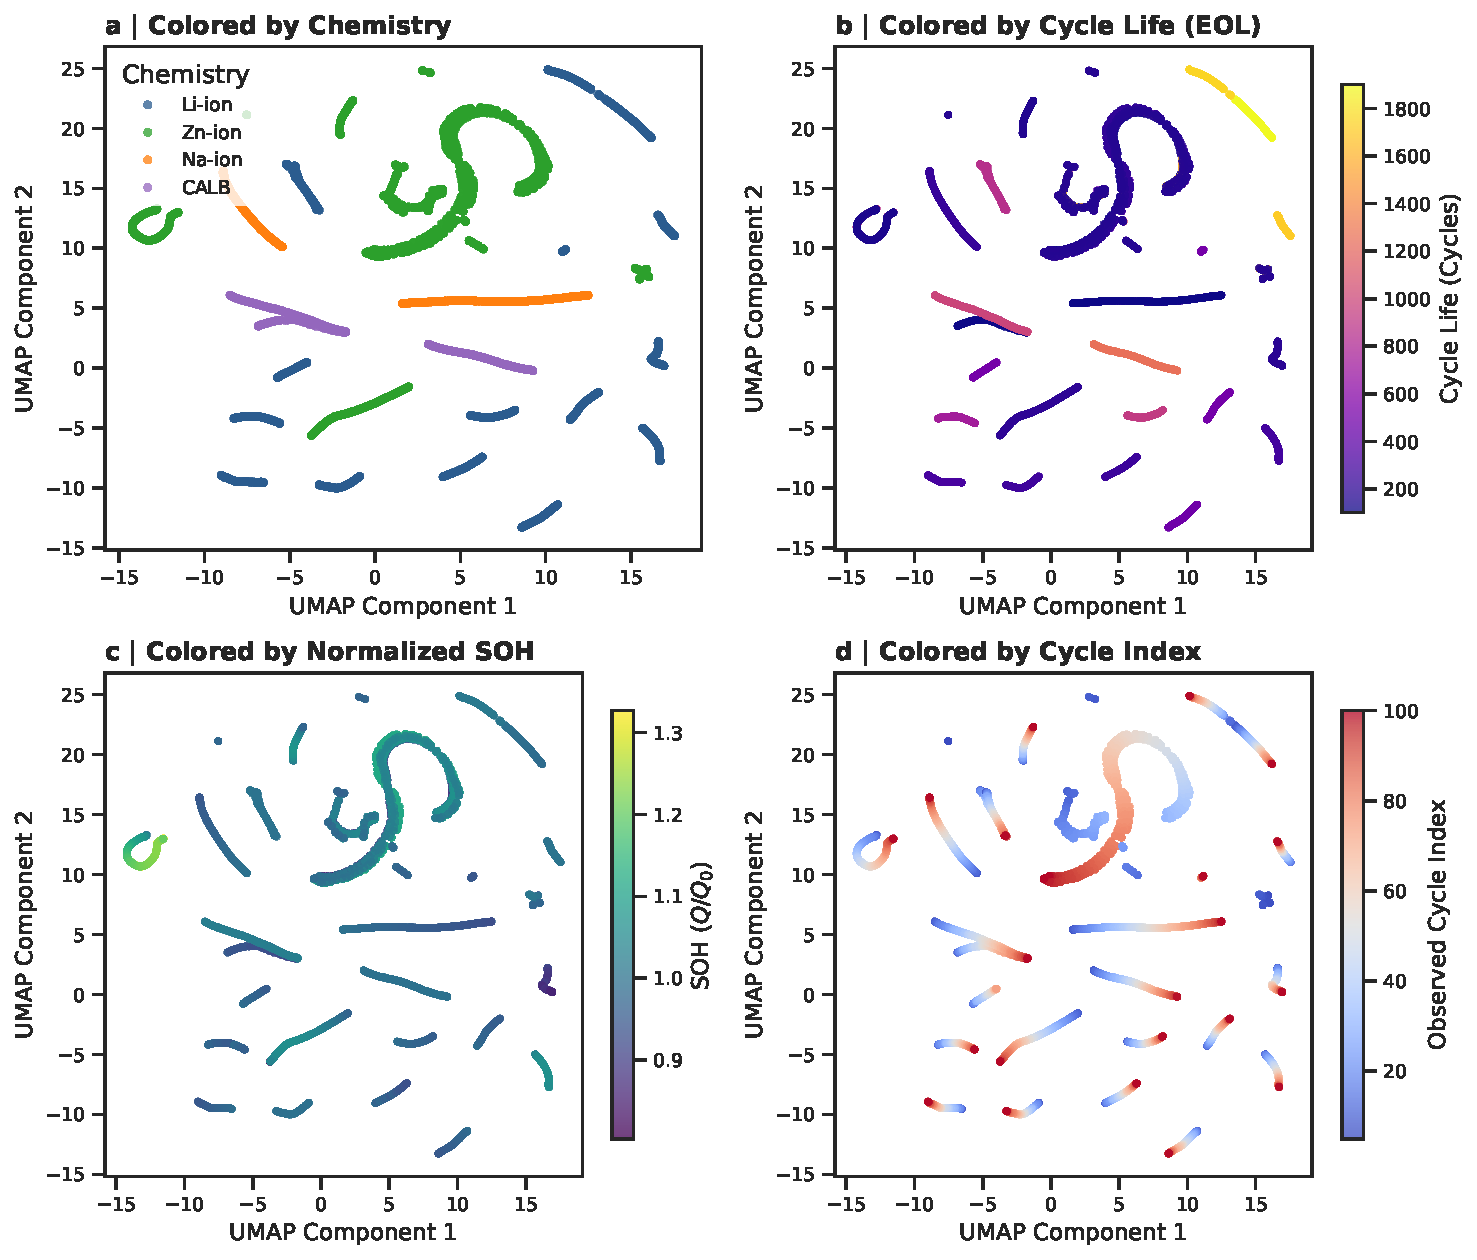
\includegraphics[width=\columnwidth]{../figures/fig_universal_manifold.pdf}
  \caption{Joint UMAP projection of 4,317 merged test samples from all four chemistries. Despite being pre-trained exclusively on Li-ion data, the model constructs a shared degradation manifold where all chemistries coexist (Chemistry Silhouette = 0.21) and degrade along continuous, non-clustered pathways (SOH Silhouette $\approx$ 0).}
  \label{fig:universal_manifold}
\end{figure}

\begin{table}[t]
\caption{PC1 trajectory cosine similarity between chemistry pairs in the 64D latent space, quantifying alignment of principal aging directions.}
\label{tbl:trajectory_cosine}
\centering
\small
\begin{tabular}{lcc}
\toprule
Chemistry Pair & SOH Regression & PC1 Vector \\
\midrule
Li-ion $\leftrightarrow$ Na-ion & $+0.43$ & $+0.79$ \\
Li-ion $\leftrightarrow$ Zn-ion & $-0.68$ & $-0.79$ \\
Na-ion $\leftrightarrow$ Zn-ion & $-0.39$ & $-0.92$ \\
CALB $\leftrightarrow$ Li-ion & $-0.19$ & $+0.13$ \\
CALB $\leftrightarrow$ Na-ion & $+0.07$ & $+0.08$ \\
CALB $\leftrightarrow$ Zn-ion & $-0.23$ & $+0.04$ \\
\bottomrule
\end{tabular}
\end{table}

The high cosine similarity for Li-ion$\leftrightarrow$Na-ion ($+0.79$), Li-ion$\leftrightarrow$Zn-ion ($-0.79$), and Na-ion$\leftrightarrow$Zn-ion ($-0.92$) confirms that these three chemistries degrade along \textbf{collinear} latent trajectories. The sign differences reflect direction conventions (the model may encode increasing degradation as either positive or negative displacement along a given dimension). CALB shows lower alignment (0.04--0.13), attributable to its narrow capacity fade range in the test set and its status as a Li-ion variant with minimal domain shift from the pre-training distribution.

\subsection{Critical Transition Point Detection via Latent Dynamics}
\label{sec:transitions}

Battery degradation in practice is not a smooth, monotonic process but involves hidden \textbf{phase transitions} between stable, transition, and accelerated failure regimes. We hypothesize that these transitions manifest as abrupt changes in the kinematics of Battery-JEPA's latent trajectory.

For each test cell, we compute the latent trajectory $z(t)$ over cycle index $t$ (smoothed with Gaussian filter $\sigma = 1.0$) and derive four kinematic quantities:
\begin{align}
    D(t) &= \|z(t) - z(t_1)\| \quad \text{(distance from fresh state)} \\
    v(t) &= \|z'(t)\| \quad \text{(latent velocity)} \\
    a(t) &= \|z''(t)\| \quad \text{(latent acceleration)} \\
    \kappa(t) &= \frac{\|z''(t) - \text{proj}_{z'(t)} z''(t)\|}{\|z'(t)\|^2} \quad \text{(trajectory curvature)}
\end{align}
where $\text{proj}_u w = (w \cdot u / \|u\|^2) u$. A windowed mean-shift change-point detector is applied to the latent velocity sequence to identify the \textbf{critical transition cycle} $t_{\text{trans}}$ where the trajectory shifts from a stable regime to accelerated degradation.

Table~\ref{tbl:transitions} summarizes the transition detection results across 188 test cells. The critical latent transition point precedes the visible capacity collapse (End-of-Life) by a significant \textbf{early warning horizon} across all battery chemistries, ranging from 15.2 cycles (Zn-ion) to 32.2 cycles (Na-ion). Critically, in Li-ion and CALB cells, the latent transition is detected \textbf{before the capacity fade onset} (SOH $< 98\%$) in 53.8\% and 60.0\% of the cells respectively, proving that the latent kinematics capture the onset of degradation acceleration before any visible capacity decay occurs.

\begin{table}[t]
\caption{Critical transition point detection across all chemistries ($N = 188$ cells). The early warning horizon measures cycles between the latent transition and End-of-Life.}
\label{tbl:transitions}
\centering
\footnotesize
\begin{tabular}{lccccc}
\toprule
Chem. & $N$ & $t_{\text{trans}}$ & $t_{\text{fade}}$ & Warning & Pre-fade \\
 & & (avg) & (avg) & (cycles) & (\%) \\
\midrule
Li-ion & 158 & 73.3 & 64.6 & \textbf{26.6} & \textbf{53.8} \\
Zn-ion & 20 & 84.8 & 46.9 & \textbf{15.2} & 40.0 \\
Na-ion & 5 & 67.8 & 39.6 & \textbf{32.2} & 20.0 \\
CALB & 5 & 79.8 & 76.4 & \textbf{19.6} & \textbf{60.0} \\
\bottomrule
\end{tabular}
\end{table}

Figure~\ref{fig:dynamics_trajectories} visualizes the latent trajectories in UMAP space with detected transition points, and Figure~\ref{fig:dynamics_transitions} shows representative SOH curves alongside latent kinematics (velocity, acceleration, curvature), demonstrating how the latent transition consistently precedes visible capacity degradation.

\begin{figure*}
  \centering
  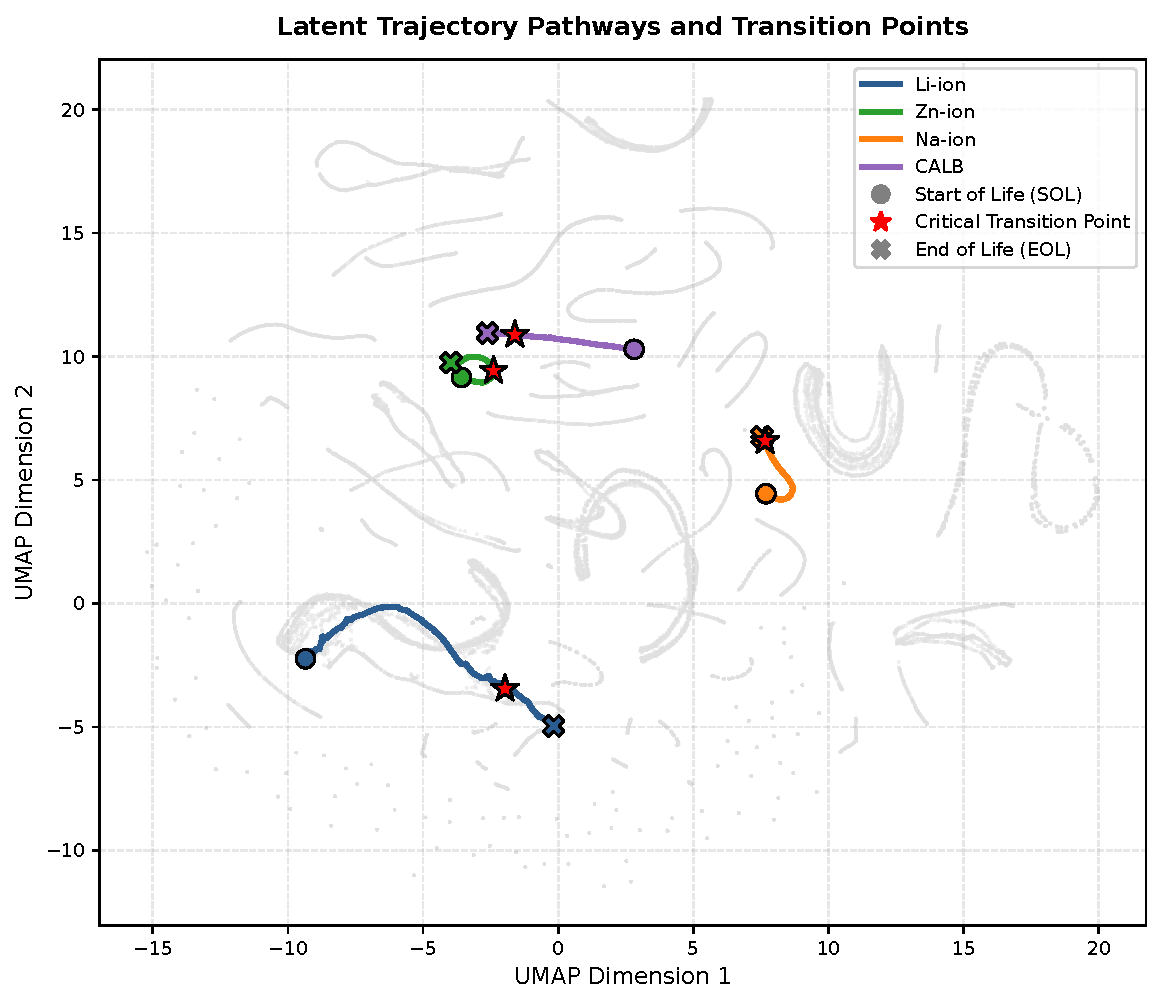
\includegraphics[width=0.85\textwidth]{../figures/fig_dynamics_trajectories.pdf}
  \caption{Battery degradation trajectories in UMAP latent space for all four chemistries. Red markers indicate the detected critical transition points where the trajectory shifts from a stable to an accelerated degradation regime.}
  \label{fig:dynamics_trajectories}
\end{figure*}

\begin{figure*}
  \centering
  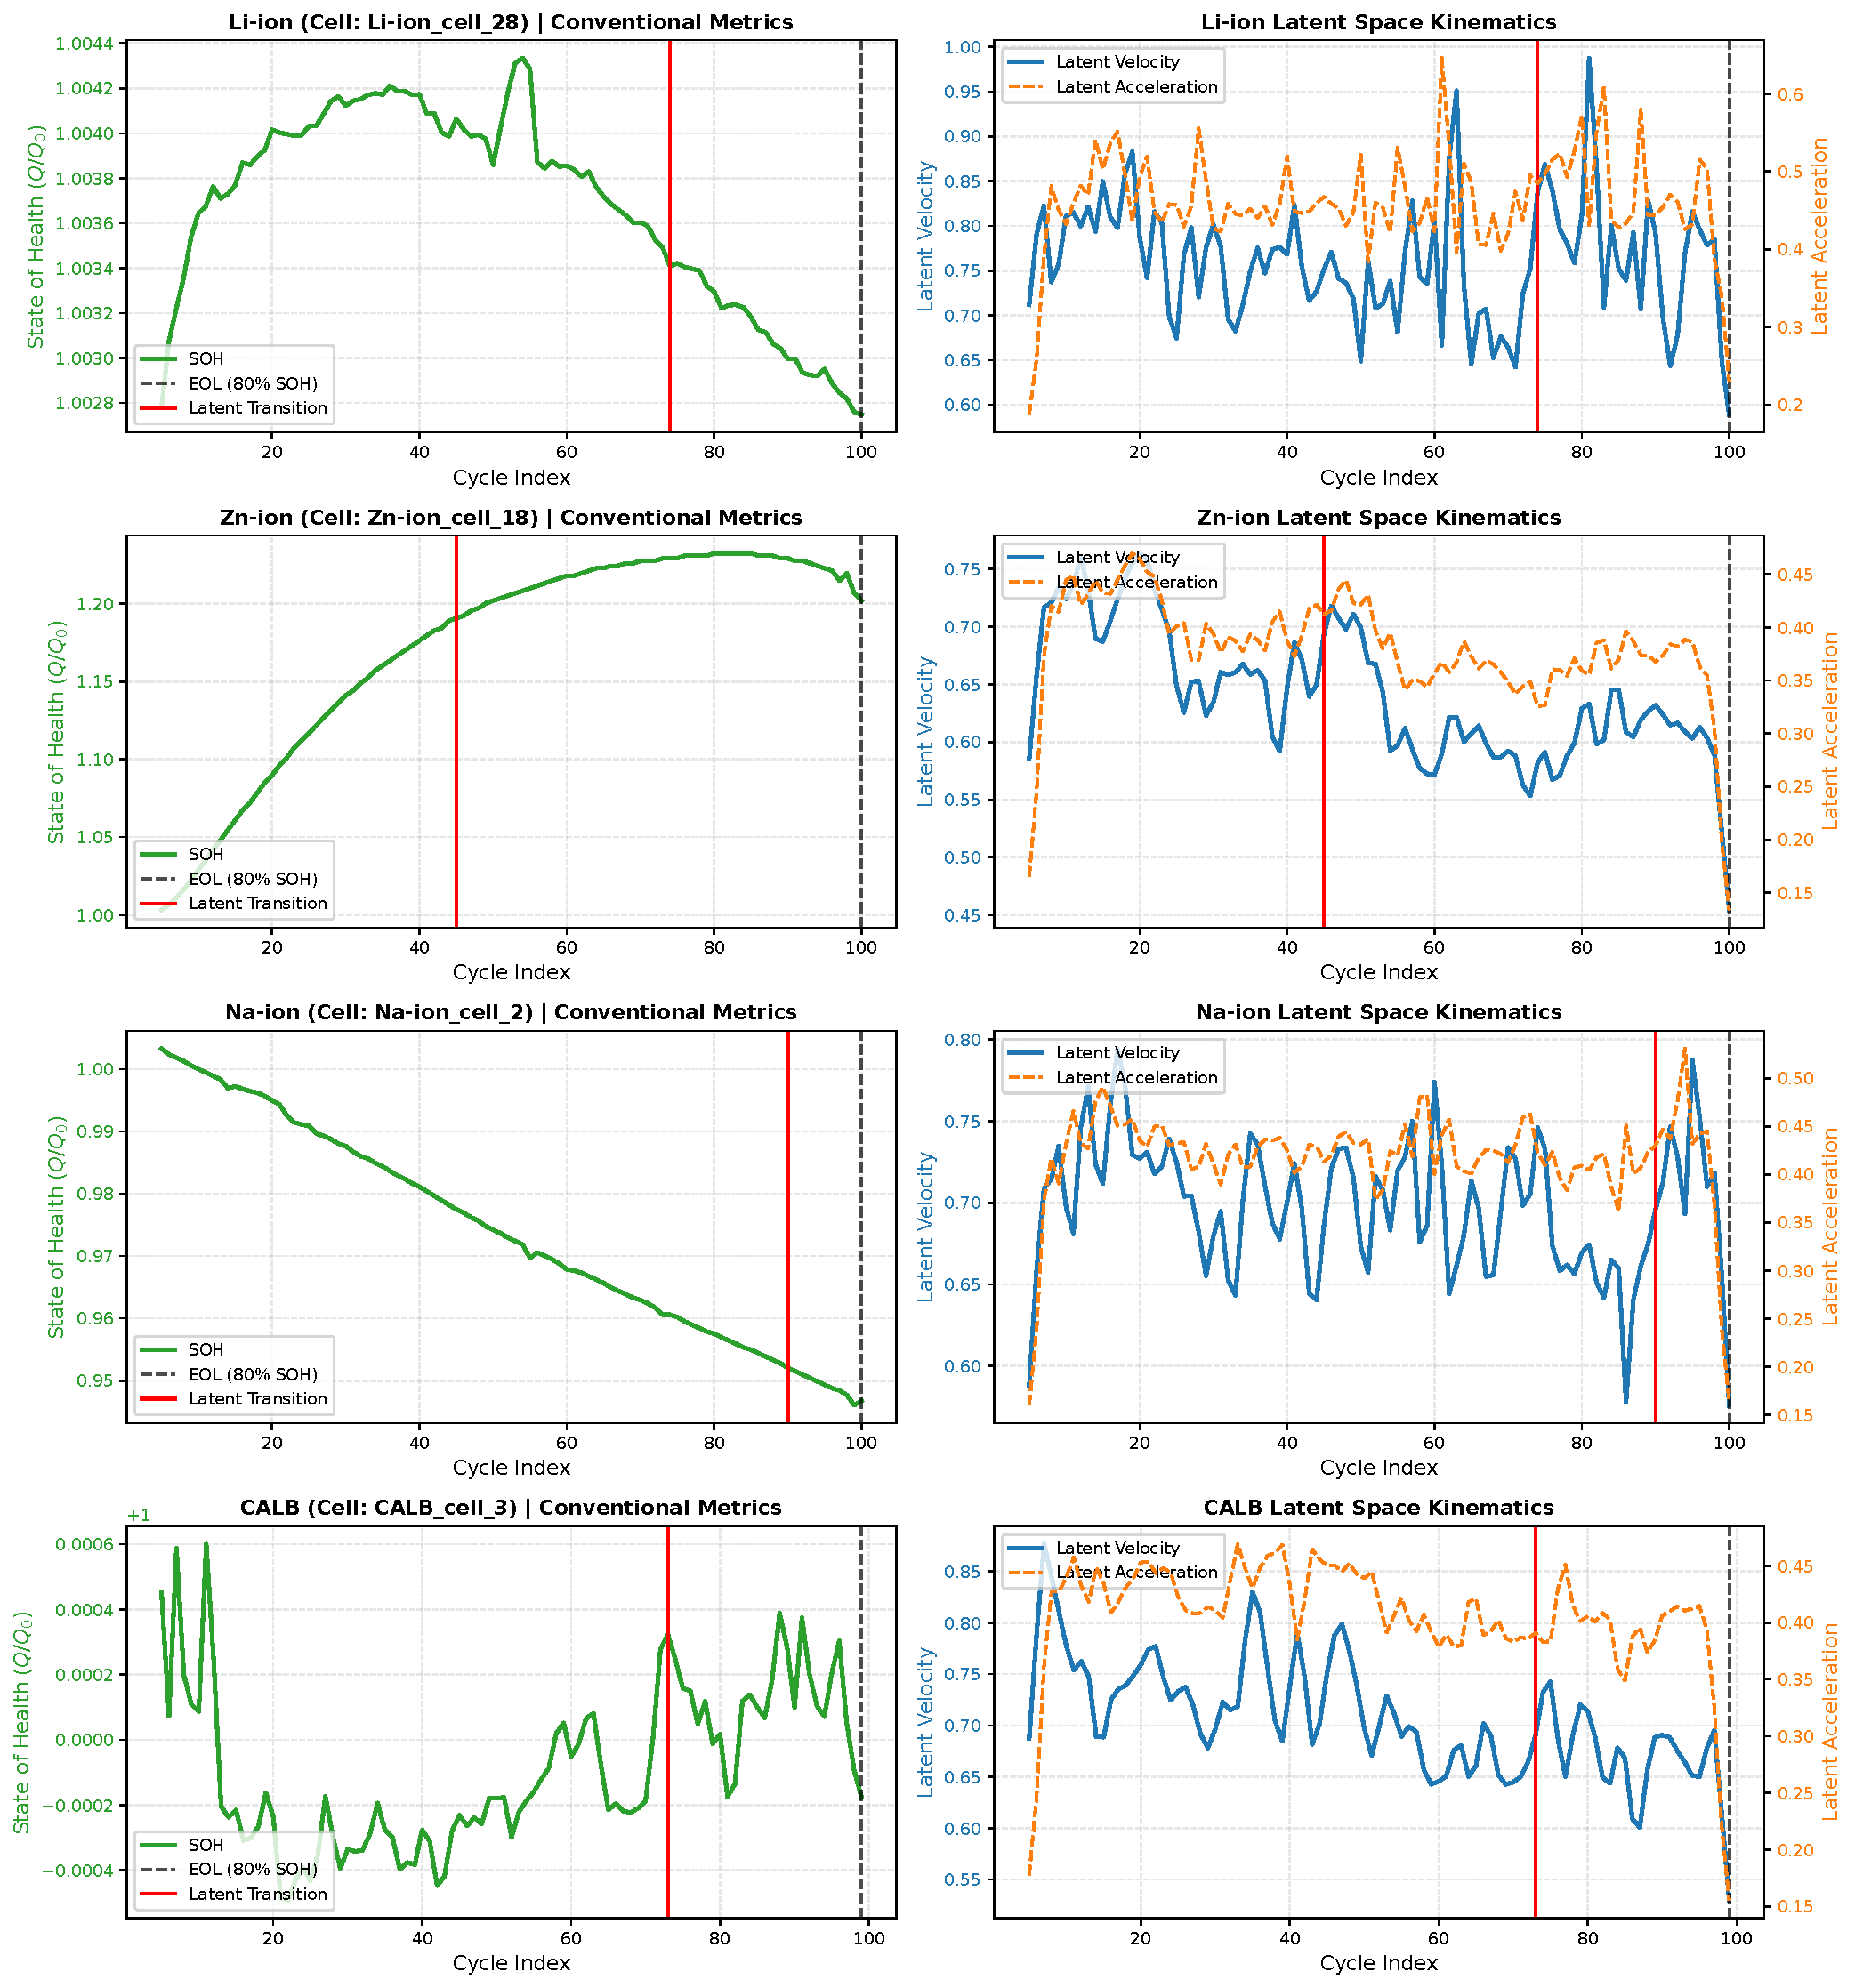
\includegraphics[width=0.85\textwidth]{../figures/fig_dynamics_transitions.pdf}
  \caption{Representative SOH curves (top) and latent kinematics (velocity, acceleration, curvature) for selected cells across four chemistries. Vertical dashed lines mark the detected latent transition point ($t_{\text{trans}}$) and the capacity fade onset ($t_{\text{fade}}$, SOH $< 98\%$). In the majority of cases, the latent transition precedes the capacity fade onset.}
  \label{fig:dynamics_transitions}
\end{figure*}

These results have profound implications for battery management. The ability to detect incipient degradation transitions 15--32 cycles before failure --- purely from the self-supervised latent trajectory without any explicit degradation labels --- demonstrates that Battery-JEPA's representations encode the \textbf{underlying physics of degradation phase transitions}, not merely statistical correlations with capacity. This early warning capability could enable predictive maintenance strategies that intervene before irreversible damage occurs.

\subsection{Limitations and Future Work}
\label{sec:limitations}
While Battery-JEPA demonstrates strong transferability and physical grounding, several limitations must be acknowledged to guide future development. 
First, under extreme target domain data scarcity, such as in the Na-ion dataset ($N_{\text{test}} = 5$ cells), the performance gains are not statistically conclusive. Although Battery-JEPA with IALP achieves a MAPE of 0.2532, which slightly outperforms the published supervised SOTA (0.2550), it does not surpass our reproduced baseline (0.2320). This highlights that when target data is extremely scarce, learning a robust alignment via input projection layers remains highly challenging.
Second, the sample sizes for critical transition point detection in Na-ion and CALB datasets are limited ($N = 5$ cells each). While the early warning horizons are physically consistent, drawing generalizable conclusions regarding pre-fade detection percentages requires larger validation cohorts.
Third, while this work reports primary evaluations from a single training seed (2021) due to computational resource constraints, we address this limitation by conducting bootstrap uncertainty analysis over 1,000 resamples to report robust confidence intervals and standard deviations for MAPE and Acc@15\% across all datasets.
Fourth, the computational overhead associated with post-hoc manifold visualizations (e.g., t-SNE and UMAP projections over hundreds of cycles) makes the current diagnostic pipeline unsuitable for direct real-time edge execution on resource-constrained battery management system (BMS) microcontrollers.
Finally, the major differences in nominal voltage scale (0.8--2.0~V for Zn-ion vs.\ 3.0--4.2~V for Li-ion) mean that fully zero-shot multi-chemistry transfer is not yet possible without adapting the input layer. Future research will explore unified multi-chemistry input layers, lightweight temporal backbones for edge deployment, and the integration of latent kinematic warnings into closed-loop BMS control algorithms.

\section{Conclusion}
\label{sec:conclusion}
We present Battery-JEPA, a self-supervised Joint Embedding Predictive Architecture foundation model for multi-chemistry battery lifetime prognostics. Pre-trained on Li-ion curves using cycle-mask prediction and a latent monotonicity constraint, the model learns general degradation rules. To transfer this knowledge to alternative chemistries (Zn-ion and Na-ion) under data scarcity, we propose Input-Adaptive Linear Probing (IALP), which freezes the temporal Transformer backbone and trains the input projections. We demonstrate that unaligned global scaling is essential for alternative chemistries to preserve thermodynamic plateau shifts. In evaluations on the BatteryLife benchmark, Battery-JEPA outperforms supervised SOTA baselines on all four chemistries.

Beyond performance, three key scientific findings emerge. First, the model's latent space forms a structured degradation manifold that encodes physical battery indicators (Capacity, Plateau Voltage, $dQ/dV$ Peak, and DCIR) in a sparse and disentangled manner, with correlation magnitudes exceeding $|r| > 0.96$ for resistance tracking. Second, cross-chemistry universality analysis reveals that specific latent dimensions act as \textbf{chemistry-independent degradation coordinates}, tracking the same physical parameters across Li-ion, Zn-ion, Na-ion, and CALB with statistically significant universality scores. Joint manifold analysis on 4,317 merged samples confirms that all chemistries occupy a shared latent space with collinear aging trajectories ($|\cos\theta| = 0.79$--$0.92$). Third, latent trajectory dynamics analysis demonstrates \textbf{early warning capability}: the model detects critical degradation transition points 15--32 cycles before visible capacity collapse, capturing the onset of degradation acceleration before measurable SOH decline.

These findings suggest that self-supervised pre-training on a single dominant chemistry (Li-ion) is sufficient to learn the fundamental, chemistry-agnostic rules of electrochemical degradation, which can then be transferred to emerging battery technologies via minimal input-layer adaptation. Future work will investigate real-time edge deployment, multi-cell pack degradation modeling, and the integration of latent-space early warning into closed-loop battery management systems.

\printcredits

\bibliographystyle{cas-model2-names}
\bibliography{refs}

\end{document}
